% !TeX program = XeLaTeX or LuaLaTeX
% !TeX encoding = UTF-8 Unicode
\documentclass[a4paper,oneside,12pt]{article}
%%%%%%%%%%%%%%%%%%%%%%%%%%%%%%%%%%%%%%%%%%%%%%%%%%%%%%%%%%%%%%%%%%%%%%%%%%%%%%%%%
%% Packages
%%%%%%%%%%%%%%%%%%%%%%%%%%%%%%%%%%%%%%%%%%%%%%%%%%%%%%%%%%%%%%%%%%%%%%%%%%%%%%%%%
\usepackage[spanish]{babel}
\usepackage{multirow}
\usepackage{amsmath}
\usepackage{fontspec}
\usepackage[xetex]{graphicx}
\usepackage{csquotes}
\usepackage{a4wide} %%Smaller margins, more text per page.
\usepackage{longtable} %%For tables that exceed a page width
\usepackage{caption} %%Pro­vides many ways to cus­tomise the cap­tions in float­ing en­vi­ron­ments like fig­ure and ta­ble
\usepackage{float} %%Im­proves the in­ter­face for defin­ing float­ing ob­jects such as fig­ures and ta­bles
\usepackage[tablegrid,nochapter]{vhistory} %%Vhis­tory sim­pli­fies the cre­ation of a his­tory of ver­sions of a doc­u­ment
\usepackage[nottoc]{tocbibind} %%Au­to­mat­i­cally adds the bib­li­og­ra­phy and/or the in­dex and/or the con­tents, etc., to the Ta­ble of Con­tents list­ing
\usepackage[toc,page]{appendix} %%The ap­pendix pack­age pro­vides var­i­ous ways of for­mat­ting the ti­tles of ap­pen­dices
\usepackage{pdfpages} %%This pack­age sim­pli­fies the in­clu­sion of ex­ter­nal multi-page PDF doc­u­ments in LATEX doc­u­ments
\usepackage[rightcaption]{sidecap} %%De­fines en­vi­ron­ments called SC­fig­ure and SCtable (anal­o­gous to fig­ure and ta­ble) to type­set cap­tions side­ways
% \usepackage{cite} %%The pack­age sup­ports com­pressed, sorted lists of nu­mer­i­cal ci­ta­tions, and also deals with var­i­ous punc­tu­a­tion and other is­sues of rep­re­sen­ta­tion, in­clud­ing com­pre­hen­sive man­age­ment of break points
\usepackage[printonlyused]{acronym} %%This pack­age en­sures that all acronyms used in the text are spelled out in full at least once. It also pro­vides an en­vi­ron­ment to build a list of acronyms used
% \usepackage[pdftex,scale={.8,.8}]{geometry} %%The pack­age pro­vides an easy and flex­i­ble user in­ter­face to cus­tomize page lay­out, im­ple­ment­ing auto-cen­ter­ing and auto-bal­anc­ing mech­a­nisms so that the users have only to give the least de­scrip­tion for the page lay­out. For ex­am­ple, if you want to set each mar­gin 2cm with­out header space, what you need is just \usep­a­ck­age[mar­gin=2cm,no­head]{ge­om­e­try}.
\usepackage{layout} %%The pack­age de­fines a com­mand \lay­out, which will show a sum­mary of the lay­out of the cur­rent doc­u­ment
\usepackage{subfigure} %%Pro­vides sup­port for the ma­nip­u­la­tion and ref­er­ence of small or ‘sub’ fig­ures and ta­bles within a sin­gle fig­ure or ta­ble en­vi­ron­ment.
\usepackage[toc]{glossaries} %%The glos­saries pack­age sup­ports acronyms and mul­ti­ple glos­saries, and has pro­vi­sion for op­er­a­tion in sev­eral lan­guages (us­ing the fa­cil­i­ties of ei­ther ba­bel or poly­glos­sia).
\usepackage[left,pagewise,modulo]{lineno} %%Adds line num­bers to se­lected para­graphs with ref­er­ence pos­si­ble through the LATEX \ref and \pageref cross ref­er­ence mech­a­nism
\usepackage[xetex,colorlinks=false,hidelinks,pdfstartview=FitV,bookmarks=true]{hyperref}%%The hy­per­ref pack­age is used to han­dle cross-ref­er­enc­ing com­mands in LATEX to pro­duce hy­per­text links in the doc­u­ment. 
\usepackage{metainfo}
\usepackage[top=1in,bottom=1in,left=1in,right=1in]{geometry}
% \usepackage[a4paper,left=2.5cm,right=2.5cm,top=\dimexpr15mm+1.5\baselineskip,bottom=2cm]{geometry}
\usepackage{geometry}
% \usepackage[pagestyles,raggedright]{titlesec}
\usepackage{etoolbox}
\usepackage{tabularx}
\usepackage{ltxtable}
\usepackage[style=ieee]{biblatex}
\bibliography{base/Docker.bib}
\usepackage[nottoc]{tocbibind}
\usepackage[official]{eurosym}
\usepackage{gensymb}
\usepackage{qrcode}
\usepackage{numprint}
\usepackage{mathtools}
\usepackage[nice]{nicefrac}
\usepackage{tikz}
\usetikzlibrary{arrows,automata,babel,positioning,calc}
\usepackage{%
    array, %%An ex­tended im­ple­men­ta­tion of the ar­ray and tab­u­lar en­vi­ron­ments which ex­tends the op­tions for col­umn for­mats, and pro­vides "pro­grammable" for­mat spec­i­fi­ca­tions
    booktabs, %%The pack­age en­hances the qual­ity of ta­bles in LATEX, pro­vid­ing ex­tra com­mands as well as be­hind-the-scenes op­ti­mi­sa­tion
    dcolumn, %%
    rotating,
    shortvrb,
    units,
    url,
    longtable,
    lscape,
    qtree,
    skmath,	
    enumitem,
    wasysym,
    mathcomp,
    titling,
    libertine,
    fancyhdr,
    microtype
}

% Necessary packages for the titlepage:
\usepackage{comment}

\newcommand{\bigO}[1]{%
  \text{\usefont{OMS}{cmsy}{m}{n}O}\left(#1\right)%
}
%%%%%%%%%%%%%%%%%%%%%%%%%%%%%%%%%%%%%%%%%%%%%%%%%%%%%%%%%%%%%%%%%%%%%%%%%%%%%%%%%
%% Java --> latex 
%%%%%%%%%%%%%%%%%%%%%%%%%%%%%%%%%%%%%%%%%%%%%%%%%%%%%%%%%%%%%%%%%%%%%%%%%%%%%%%%%
\setmonofont{Fira Code}[
  Contextuals=Alternate,
  Ligatures = {Common,Rare}
]
\usepackage{letltxmacro}
\LetLtxMacro\oldttfamily\ttfamily
\DeclareRobustCommand{\ttfamily}{\oldttfamily\csname ttsize\endcsname}
\newcommand{\settttsize}[1]{\def\ttsize{#1}}%
\usepackage{lstfiracode}
\usepackage{listings}

\lstset{ %
  backgroundcolor=\color{white},   % Indica el color de fondo; necesita que se añada \usepackage{color} o \usepackage{xcolor}
  basicstyle=\footnotesize\ttfamily,        % Fija el tamaño del tipo de letra utilizado para el código
  breakatwhitespace=false,         % Activarlo para que los saltos automáticos solo se apliquen en los espacios en blanco
  inputencoding=utf8,
  breaklines=true,                 % Activa el salto de línea automático
  captionpos=b,                    % Establece la posición de la leyenda del cuadro de código
  commentstyle=\color{darkgreen},    % Estilo de los comentarios
  extendedchars=true,              % Permite utilizar caracteres extendidos no-ASCII; solo funciona para codificaciones de 8-bits; para UTF-8 no funciona. En xelatex necesita estar a true para que funcione.
  frame=single,	                   % Añade un marco al código
  keepspaces=true,                 % Mantiene los espacios en el texto. Es útil para mantener la indentación del código(puede necesitar columns=flexible).
  columns=flexible,
  keywordstyle=\color{darkorange},       % estilo de las palabras clave
  numbers=left,                    % Posición de los números de línea (none, left, right).
  numbersep=5pt,                   % Distancia de los números de línea al código
  numberstyle=\small\color{gray}, % Estilo para los números de línea
  rulecolor=\color{black},         % Si no se activa, el color del marco puede cambiar en los saltos de línea entre textos que sea de otro color, por ejemplo, los comentarios, que están en verde en este ejemplo
  showspaces=false,                % Si se activa, muestra los espacios con guiones bajos; sustituye a 'showstringspaces'
  showstringspaces=false,          % subraya solamente los espacios que estén en una cadena de esto
  showtabs=false,                  % muestra las tabulaciones que existan en cadenas de texto con guión bajo
  stringstyle=\color{darkgreen},     % Estilo de las cadenas de texto
  style=FiraCodeStyle,
  identifierstyle=\color{blue},
  tabsize=4,	                   % Establece el salto de las tabulaciones a 2 espacios
  title=\lstname,                   % muestra el nombre de los ficheros incluidos al utilizar
  caption=\lstname,
  literate={á}{{\'a}}1 {é}{{\'e}}1 {í}{{\'{\i}}}1 {ó}{{\'o}}1 {ú}{{\'u}}1 {Á}{{\'A}}1 {É}{{\'E}}1 {Í}{{\'I}}1 {Ó}{{\'O}}1 {Ú}{{\'U}}1 {ü}{{\"u}}1 {Ü}{{\"U}}1 {ñ}{{\~n}}1 {Ñ}{{\~N}}1 {¿}{{?``}}1 {¡}{{!``}}1 {º}{\textdegree}1,
  postbreak=\mbox{\textcolor{red}{$\hookrightarrow$}\space},
}
\lstdefinelanguage{docker}{
  keywords={FROM, RUN, COPY, ADD, ENTRYPOINT, CMD,  ENV, ARG, WORKDIR, EXPOSE, LABEL, USER, VOLUME, STOPSIGNAL, ONBUILD, MAINTAINER},
  keywordstyle=\color{blue}\bfseries,
  identifierstyle=\color{black},
  sensitive=false,
  comment=[l]{\#},
  commentstyle=\color{purple}\ttfamily,
  stringstyle=\color{red}\ttfamily,
  morestring=[b]',
  morestring=[b]"
}

\lstdefinelanguage{docker-compose}{
  keywords={image, environment, ports, container_name, ports, volumes, links},
  keywordstyle=\color{blue}\bfseries,
  identifierstyle=\color{black},
  sensitive=false,
  comment=[l]{\#},
  commentstyle=\color{purple}\ttfamily,
  stringstyle=\color{red}\ttfamily,
  morestring=[b]',
  morestring=[b]"
}
\lstdefinelanguage{docker-compose-2}{
  keywords={version, volumes, services},
  keywordstyle=\color{blue}\bfseries,
  keywords=[2]{image, environment, ports, container_name, ports, links, build},
  keywordstyle=[2]\color{olive}\bfseries,
  identifierstyle=\color{black},
  sensitive=false,
  comment=[l]{\#},
  commentstyle=\color{purple}\ttfamily,
  stringstyle=\color{red}\ttfamily,
  morestring=[b]',
  morestring=[b]"
}
\lstdefinestyle{C}{%
  language=C,                 % El lenguaje del código
  otherkeywords={__attribute__, __interrupt__, inline, asm, uint8_t, uint16_t,%
  uint32_t, uint64_t, time_t, size_t, servo_t, motor_t, Nop,%
  point_t, angle_t, double64_t, int_fast64_t, bool, true, false, stdbool, stdint,%
  stdlib, stddef, NULL}           % Si se quieren añadir otras palabras clave al lenguaje
}
\lstdefinestyle{Python}{%
  language=Python
}

\lstdefinestyle{Ada}{%
  language=Ada
}
\lstdefinestyle{bash}{%
  language=bash,
  otherkeywords={sudo,chmod,chown,chgrp,ls,mkdir,touch,useradd,groupadd,usermod}
}
\lstdefinestyle{R}{%
  language=R,
  otherkeywords={0,1,2,3,4,5,6,7,8,9},
  morekeywords={TRUE,FALSE},
  deletekeywords={data,frame,length,as,character,time,ts}
}
\lstdefinestyle{Dockerfile}{%
  language=Docker,
  showstringspaces=false,
  commentstyle=\color{red},
  keywordstyle=\color{blue},
  inputencoding=utf8,
  extendedchars=true
}
\lstdefinestyle{docker-compose}{%
  language=docker-compose-2,
  showstringspaces=false,
  commentstyle=\color{red},
  keywordstyle=\color{blue},
  inputencoding=utf8,
  extendedchars=true
}
\usepackage{xcolor}
\definecolor{pblue}{rgb}{0.13,0.13,1}
\definecolor{pgreen}{rgb}{0,0.5,0}
\definecolor{pred}{rgb}{0.9,0,0}
\definecolor{pgrey}{rgb}{0.46,0.45,0.48}
\definecolor{darkgreen}{rgb}{0.0, 0.4, 0.0}
\definecolor{darkorange}{rgb}{1.0, 0.55, 0.0}
% \usepackage{inconsolata}
%%%%%%%%%%%%%%%%%%%%%%%%%%%%%%%%%%%%%%%%%%%%%%%%%%%%%%%%%%%%%%%%%%%%%%%%%%%%%%%%%
% \setlength{\parindent}{0pt}
\setlength{\parskip}{.5\baselineskip}
%% Checkmark symbols
\usepackage{pifont}
\newcommand{\cmark}{\ding{51}}%
\newcommand{\xmark}{\ding{55}}%
\newcommand{\done}{\rlap{$\square$}{\raisebox{2pt}{\large\hspace{1pt}\cmark}}%
\hspace{-2.5pt}}
\newcommand{\wontfix}{\rlap{$\square$}{\large\hspace{1pt}\xmark}}
%%%%%%%%%%%%%%%%%%%%%%%%%%%%%%%%%%%%%%%%%%%%%%%%%%%%%%%%%%%%%%%%%%%%%%%%%%%%%%%%%
%% Creation of the header
%%%%%%%%%%%%%%%%%%%%%%%%%%%%%%%%%%%%%%%%%%%%%%%%%%%%%%%%%%%%%%%%%%%%%%%%%%%%%%%%%
\patchcmd{\chapter}{plain}{short}{}{} %$ <-- the header on chapter 1
\addto\captionsspanish{%
  \renewcommand\appendixname{Anexo}
  \renewcommand\appendixpagename{Anexos}
}
\newcolumntype{s}{>{\hsize=.5\hsize\linewidth=\hsize}X}
\newcolumntype{b}{>{\hsize=.75\hsize}X}
\newcommand{\heading}[1]{\multicolumn{1}{c}{#1}}
\newcolumntype{L}[1]{>{\hsize=#1\hsize\raggedright\arraybackslash}X}%
\newcolumntype{R}[1]{>{\hsize=#1\hsize\raggedleft\arraybackslash}X}%
\newcolumntype{C}[1]{>{\hsize=#1\hsize\centering\arraybackslash}X}%

\DeclareMathOperator{\atantwo}{atan2}

\DeclareMathOperator{\arctantwo}{arctan2}
%%%%%%%%%%%%%%%%%%%%%%%%%%%%%%%%%%%%%%%%%%%%%%%%%%%%%%%%%%%%%%%%%%%%%%%%%%%%%%%%%
%% DOCUMENT
%%%%%%%%%%%%%%%%%%%%%%%%%%%%%%%%%%%%%%%%%%%%%%%%%%%%%%%%%%%%%%%%%%%%%%%%%%%%%%%%%
\author{Javier Alonso Silva}
\title{Análisis de contenedores Docker}
\date{2021}
\pagestyle{fancy}
\fancyhf{}
\fancyhfoffset[L]{1cm} % left extra length
\fancyhfoffset[R]{1cm} % right extra length
\rhead{2021}
\chead{\thetitle}
\lhead{\slshape\nouppercase{\leftmark}}
\cfoot{\thepage}
\pagenumbering{roman}

\begin{document}

\settttsize{\footnotesize}
\ActivateVerbatimLigatures
% To add this template to the main.tex file, just add the command "\include{titlePageSLU} after "\begin{docuemnt}" in the main.tex file


% In this segment, enter the desired data to be shown at the title page
\newcommand{\thesisAuthor}{\theauthor}
\newcommand{\thesisTitle}{\thetitle}
\newcommand{\thesisSubTitle}{y sus implicaciones de seguridad}
\newcommand{\thesisTitleTranslated}{Translated Headline}
\newcommand{\thesisDegree}{Seguridad en Sistemas y Redes}
\newcommand{\university}{Universidad Politécnica de Madrid}
\newcommand{\thesisPlaceDate}{\thedate}

%------------------------------------------------------------------------------
\begin{titlepage}
\thispagestyle{empty}

% Use this line of code if both SLU loggo and company/other institution loggo is desired. The positions are possible to change with the \hspace and \vspace syntax.
\begin{figure} [H]
\vspace{-2cm}
 \centering
\begin{minipage}[t]{.45\linewidth}
  \raggedright
  % Upload and include SLU loggo here:
  \hspace*{-2cm}
\includegraphics[width=\linewidth]{upmlogo.png}
  
\end{minipage}%
  \begin{minipage}[t]{.45\linewidth}
  \vspace{-3.3cm}
 \raggedleft
% Upload and include other loggo here (loggo of wikipedia is used as an example):
 \hspace*{1cm}
\includegraphics[width =0.5\textwidth]{dockerlogo.png} \hspace*{-1cm}
 
\end{minipage}
\end{figure}


% If only the logo for SLU is desired, delete "\begin{comment}" and "\end{comment}" to use this line of code:
\begin{comment}
\begin{figure}
\vspace{-3cm}
    \hspace*{-2cm}\includegraphics[width = 0.3\textwidth]{slu_logo_webb.png}\hspace*{-2cm}
\end{figure}
\end{comment}


% Adds background picture. Delete code if no background picture is wanted.
\begin{tikzpicture}[overlay, remember picture]
\node[anchor=south west, 
      xshift=-0.2cm, 
      yshift=-0.2cm] 
     at (current page.south west)
     {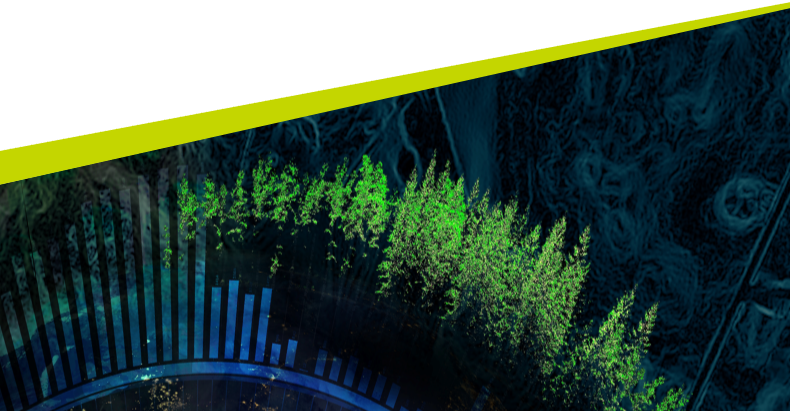
\includegraphics[width = 1.8\textwidth, height = 9cm]{background.png}}; 
\end{tikzpicture}


\vspace{1cm}
\par
\noindent
\Huge
\textbf{\thesisTitle}
\vspace{0.2cm}
\LARGE
\par
\noindent
- \thesisSubTitle\\
\rule[0.3cm]{\linewidth}{2pt}
\Large

% Delete this line if no translation is desired
% \noindent
% \textit{\thesisTitleTranslated}

\vspace{2cm}
\noindent
\LARGE
\thesisAuthor\\
\vspace{4 cm}
\small
\par \noindent
\thesisDegree
\par \noindent
\university
% \par \noindent
% \faculty
% \par \noindent
% \company
\par \noindent
\thesisPlaceDate

\end{titlepage}

\newpage
\begin{abstract}
  TO--DO
\end{abstract}

\newpage
\tableofcontents
\newpage
\pagenumbering{arabic}

\section{Introducción}
La era tecnológica ha avanzado en los últimos años a pasos agigantados, y las
demandas del sector han crecido junto a ella. No hace más de 200 años se ``descubría''
la electricidad; hace 90 años nacía la primera computadora básica capaz de realizar
operaciones aritméticas; hace 70 años nacía el transistor que sustituyó las
válvulas de vacío (figura \ref{fig:transistor}); y desde entonces, el crecimiento
ha sido exponencial \cite{HistoryTechnologyTimeline}.

\begin{figure}[H]
    \centering
    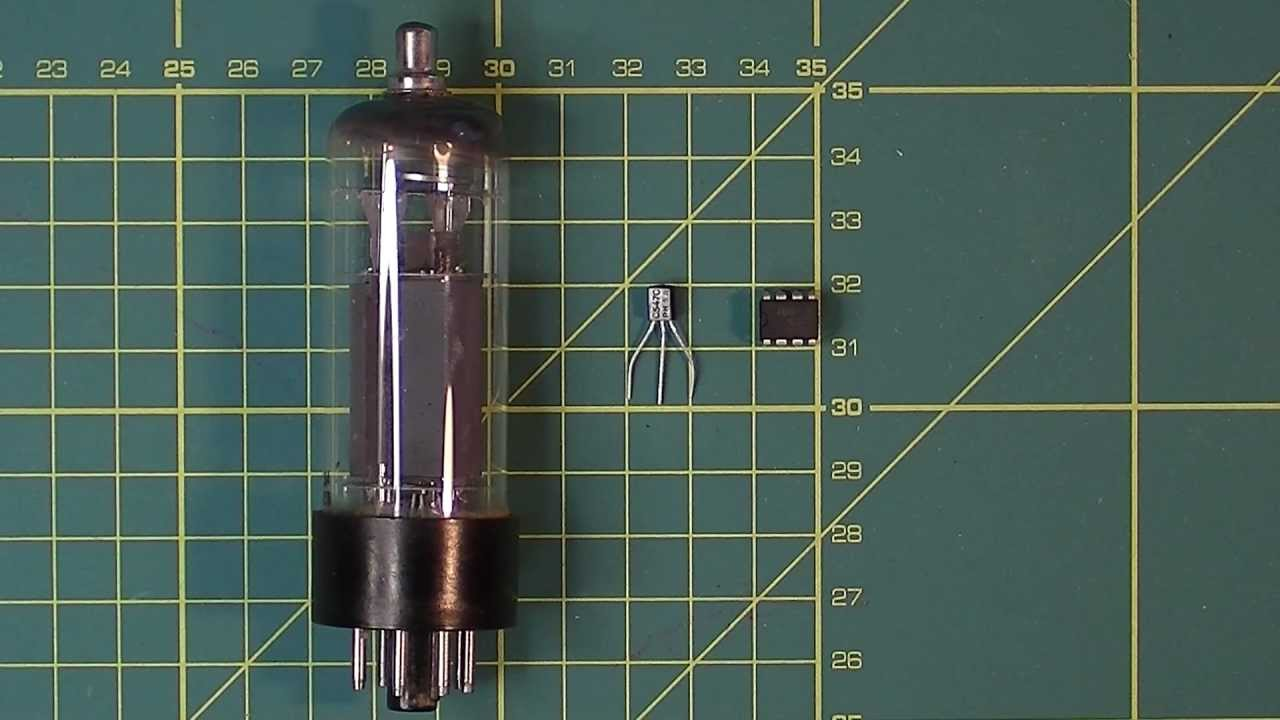
\includegraphics[width=.7\linewidth]{pictures/transistor-vs-valve.jpg}
    \caption{Comparativa de una válvula de vacío (izquierda) frente a un transistor (centro) y un circuito integrado (derecha).}
    \label{fig:transistor}
\end{figure}

Otro de los ejemplos de tecnologías que han crecido exponencialmente son los dispositivos
de almacenamiento, donde no hacía más de 20 años las capacidades máximas se estimaban
en torno a los MB (megabytes) y ahora se hablan de EB (exabytes) \cite{EvolutionDataStorage}.
Esta evolución es muy representativa también a nivel económico, ya que el coste del
almacenamiento ha ido bajando a medida pasaba el tiempo, así como el espacio físico
que ocupan los dispositivos (figura \ref{fig:disk-evolution}):

\begin{figure}[H]
    \centering
    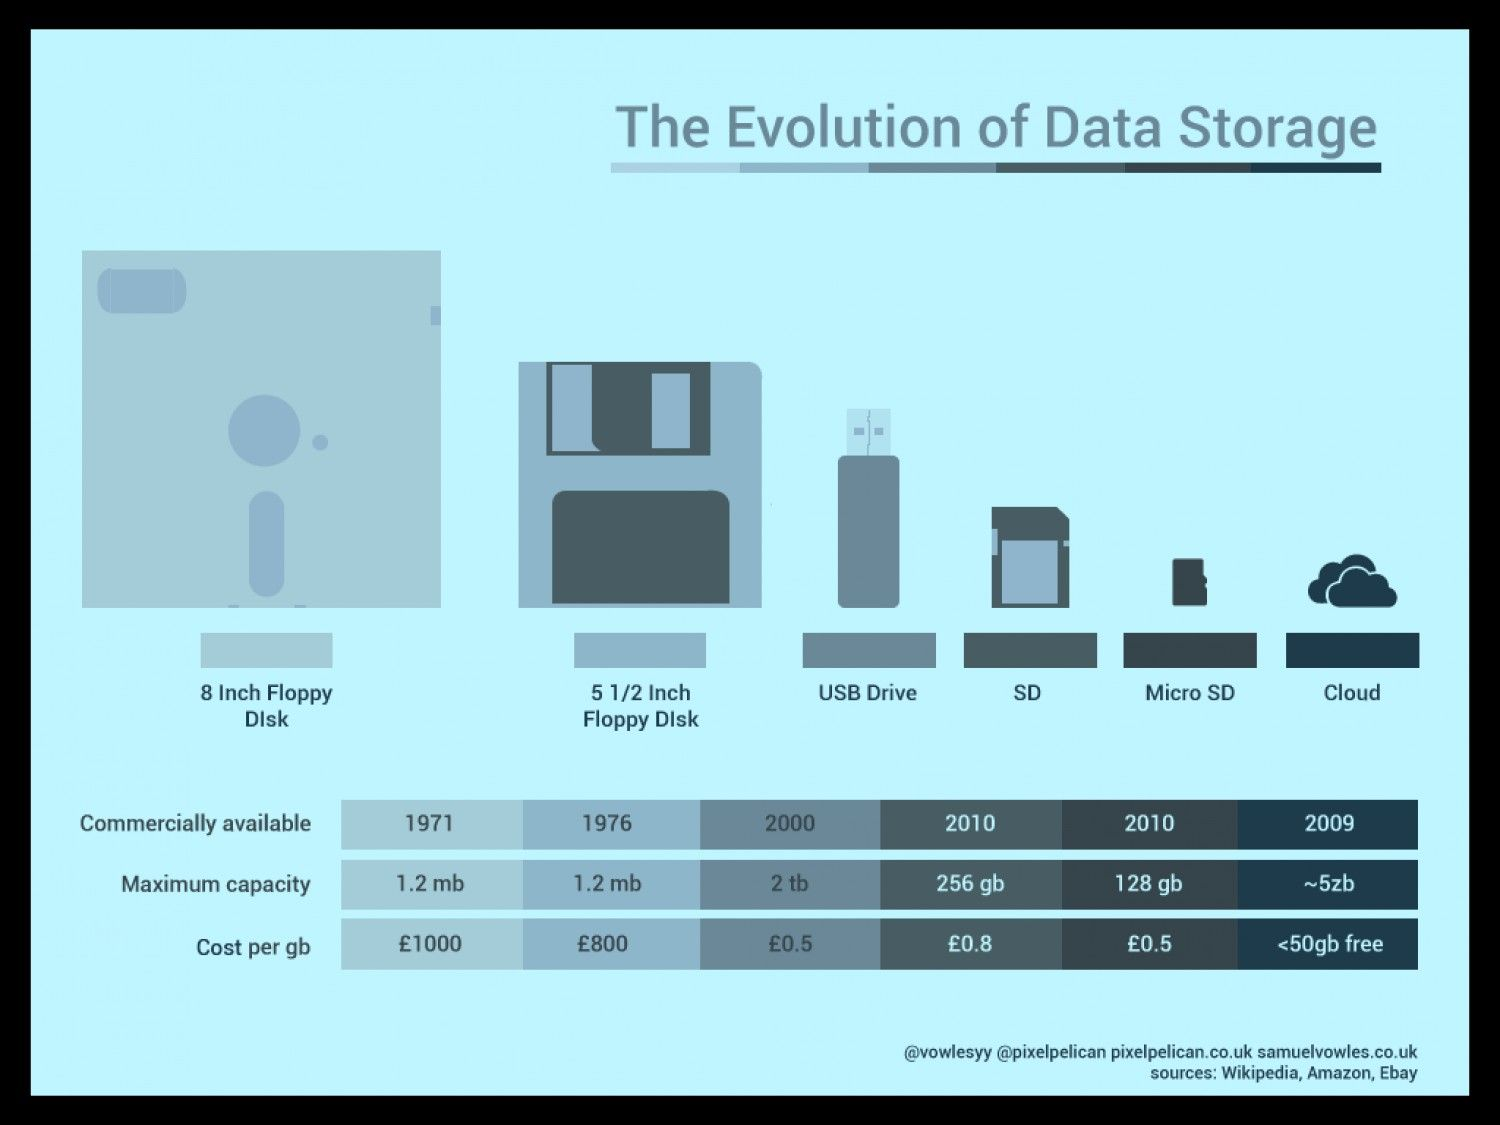
\includegraphics[width=.65\linewidth]{pictures/disk-evo.jpg}
    \caption{Evolución del espacio de almacenamiento en términos económicos y cuantitativos \cite{wecomputingtechStorageDevicesLondon}.}
    \label{fig:disk-evolution}
\end{figure}

Finalmente, el gran salto tecnológico se ha producido con la aparición de Internet y
las comunicaciones ya no eran únicamente personales sino entre dispositivos. En relación
con el punto anterior, la aparición de Internet ha permitido descentralizar el espacio
donde ya el usuario no guarda su información en su equipo personal sino en un clúster
de servidores distribuidos a nivel mundial al cual accede, de forma simultánea,
desde Internet y desde cualquier dispositivo. Así, lo que comenzó como una red de
conexión de unos pocos usuarios ha acabado convirtiéndose en la red global que
todos usamos y que conecta más de 4 billones de dispositivos (figura \ref{fig:internet-evo}).

\begin{figure}[H]
    \centering
    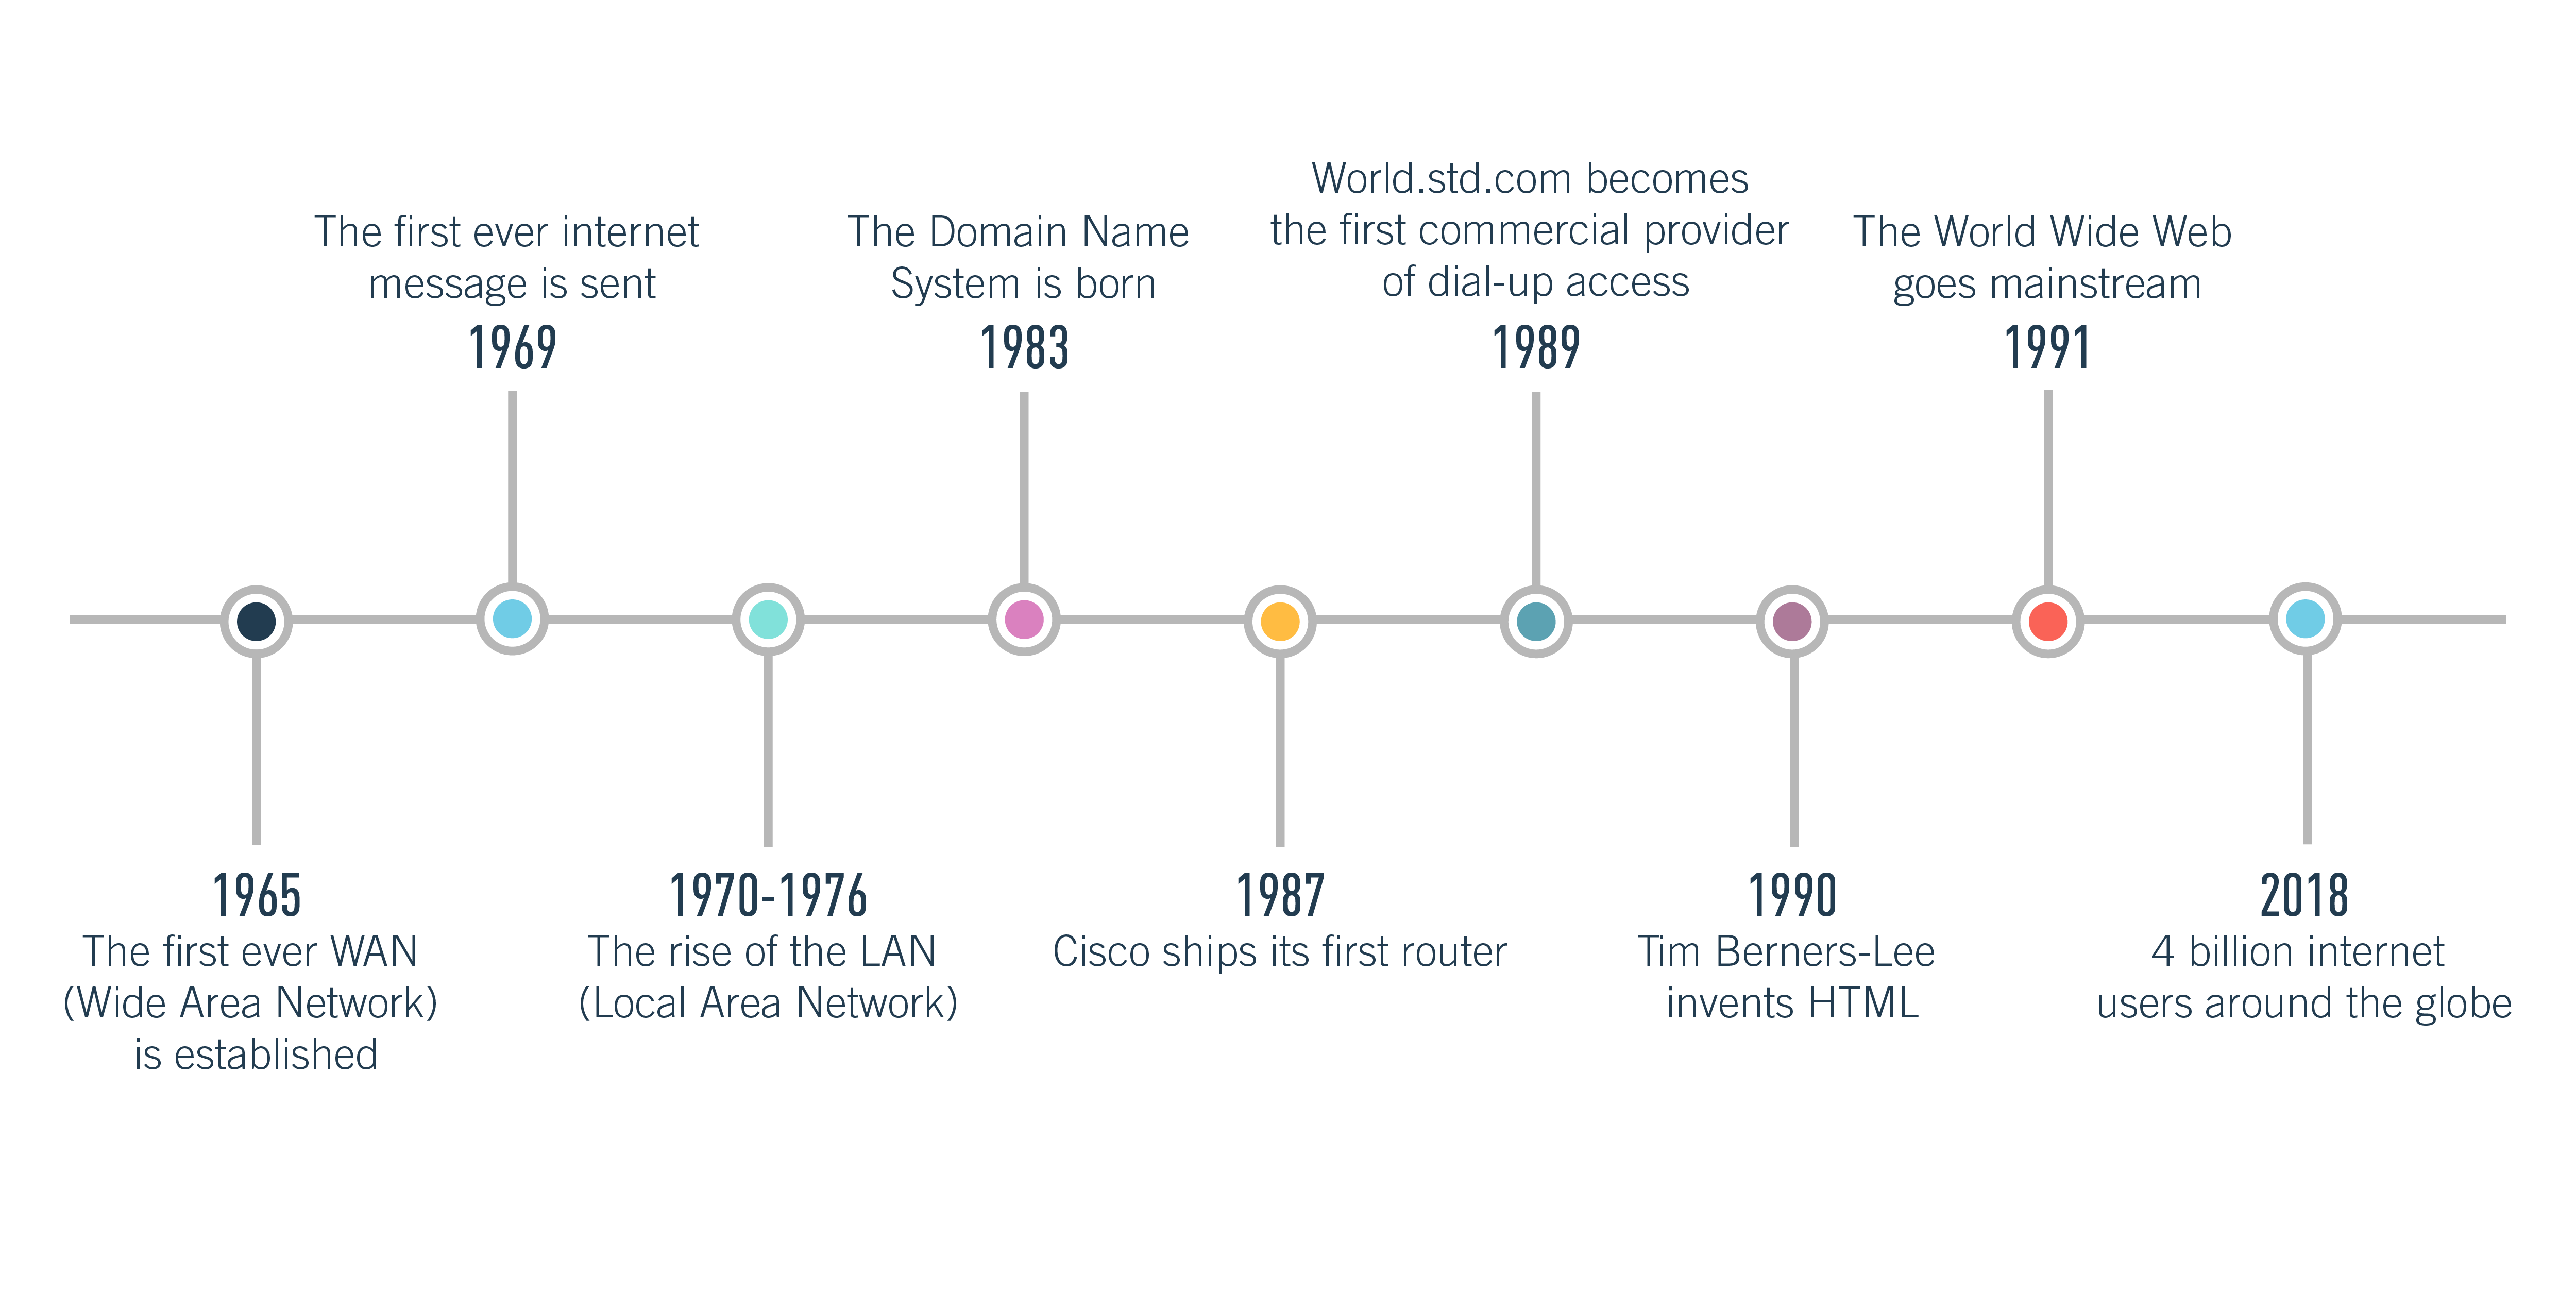
\includegraphics[width=.9\linewidth]{pictures/internet-timeline.png}
    \caption{Evolución de Internet a lo largo del tiempo, hasta llegar a hoy \cite{HowBecomeWeb}.}
    \label{fig:internet-evo}
\end{figure}

El problema a esto es evidente: con una mayor capacidad de cómputo, con más opciones
de comunicación y con más posibilidad de almacenar datos, los requisitos de las
aplicaciones van creciendo y creciendo y cada vez son más complejos de satisfacer,
no necesariamente a nivel \textit{hardware} (que por lo general suele acompañar)
sino a nivel \textit{software}. Como las aplicaciones se orientan a los usuarios
es necesario añadir capas de abstracción (como el sistema operativo) para facilitar
la labor a la persona. Sin embargo, cada capa nueva que se añade dificulta las tareas
de despliegue y mantenimiento dado que existe una gran variedad de combinaciones
\textit{hardware} y cada una puede estar con un sistema operativo distinto.

Por otra parte, la extensión de dependencias y posible incompatibilidad entre ellas
suele desembocar en el uso de versiones desactualizadas de una librería ya que tendríamos
``paquetes rotos''. Esto es tan común que tiene hasta su propio
término coloquial ``\textit{dependency hell}'' \cite{DependencyHell2021}. Contar con
dependencias obsoletas que ya han cumplido con su ciclo de vida \textit{software}
conlleva unas implicaciones de seguridad bastante severas:

\begin{itemize}
    \item Si un \textit{software} no ha mejorado a lo largo del tiempo, existe una
          malicia humana que puede aprovecharse de distintos \textit{exploits}
          existentes y comprometan nuestra aplicación.
    \item Un \textit{software} no actualizado puede tener implicaciones directas
          sobre el sistema en que se ejecuta, pudiendo producir fallos en el mismo.
          Esto se debe principalmente a que el \textit{hardware} sigue mejorando y
          creciendo y un \textit{software} antiguo puede presentar \textit{bugs}
          en dispositivos modernos que no presentaría en antiguos.
    \item Un \textit{software} no actualizado puede comprometer otros elementos del
          sistema en que se ejecuta. Por ejemplo, una aplicación `A' hace uso de dicho \textit{software}
          y una aplicación `B' también. Sin embargo, la última aplicación se ha diseñado
          para trabajar con la última versión del \textit{software} pero la aplicación
          `A' solo puede funcionar con una versión antigua e insegura. Por consiguiente,
          pese a que la aplicación `B' funcionaría correctamente el hecho de usar una
          versión antigua e insegura del \textit{software} compromete directamente al
          sistema y a la aplicación.
\end{itemize}

Es por eso que existen alternativas como ``\texttt{chroot}'' y máquinas virtuales para
subsanar estos problemas. Sin embargo, en los últimos años ha aparecido una herramienta
muy sonada y con gran éxito: Docker y los contenedores.
\subsection{¿Qué es Docker?}
Docker es una plataforma abierta diseñada para el desarrollo, despliegue y ejecución
de aplicaciones \cite{DockerOverview2021}. La idea fundamental que reside detrás de
Docker es la de separar la infraestructura de las aplicaciones de manera que se pueda
entregar el \textit{software} rápidamente.

Por debajo, Docker ofrece una plataforma que otorga la habilidad de empaquetar y
ejecutar las aplicaciones en un entorno aislado llamado ``contenedor'' (\textit{container}).
Entre otras características, un contenedor permite ejecutar una aplicación de forma
segura sobre el host en cuestión. La pregunta que surge es, ¿qué es un contenedor?

\subsubsection*{Contenedores}
Un contenedor es una unidad estándar \textit{software} que empaqueta código y todas
sus dependencias de manera que la aplicación se ejecuta rápidamente y de forma fiable
bajo múltiples entornos de ejecución \cite{WhatContainerApp}. Una imagen Docker
es un paquete ligero, independiente y ejecutable que incluye absolutamente todo
lo necesario para poder ejecutar una aplicación: desde el código en sí hasta el
\textit{runtime}, herramientas del sistema, librerías y configuraciones.

Durante la ejecución, una imagen se convierte en un contenedor que se ejecuta sobre
la máquina Docker (\textit{Docker Engine}), la cual se encuentra disponible en 
entornos Linux y Windows.

Al fin y al cabo, los contenedores nos aseguran que una aplicación que hemos 
desarrollado se va a ejecutar de la misma manera en una máquina u otra. El uso del
motor Docker permite ejecutar múltiples contenedores sobre un mismo anfitrión
sin añadir demasiada carga en el sistema e indiferentemente de la infraestructura
que exista por debajo (figura \ref{fig:docker-containers-rt}):

\begin{figure}[H]
    \centering
    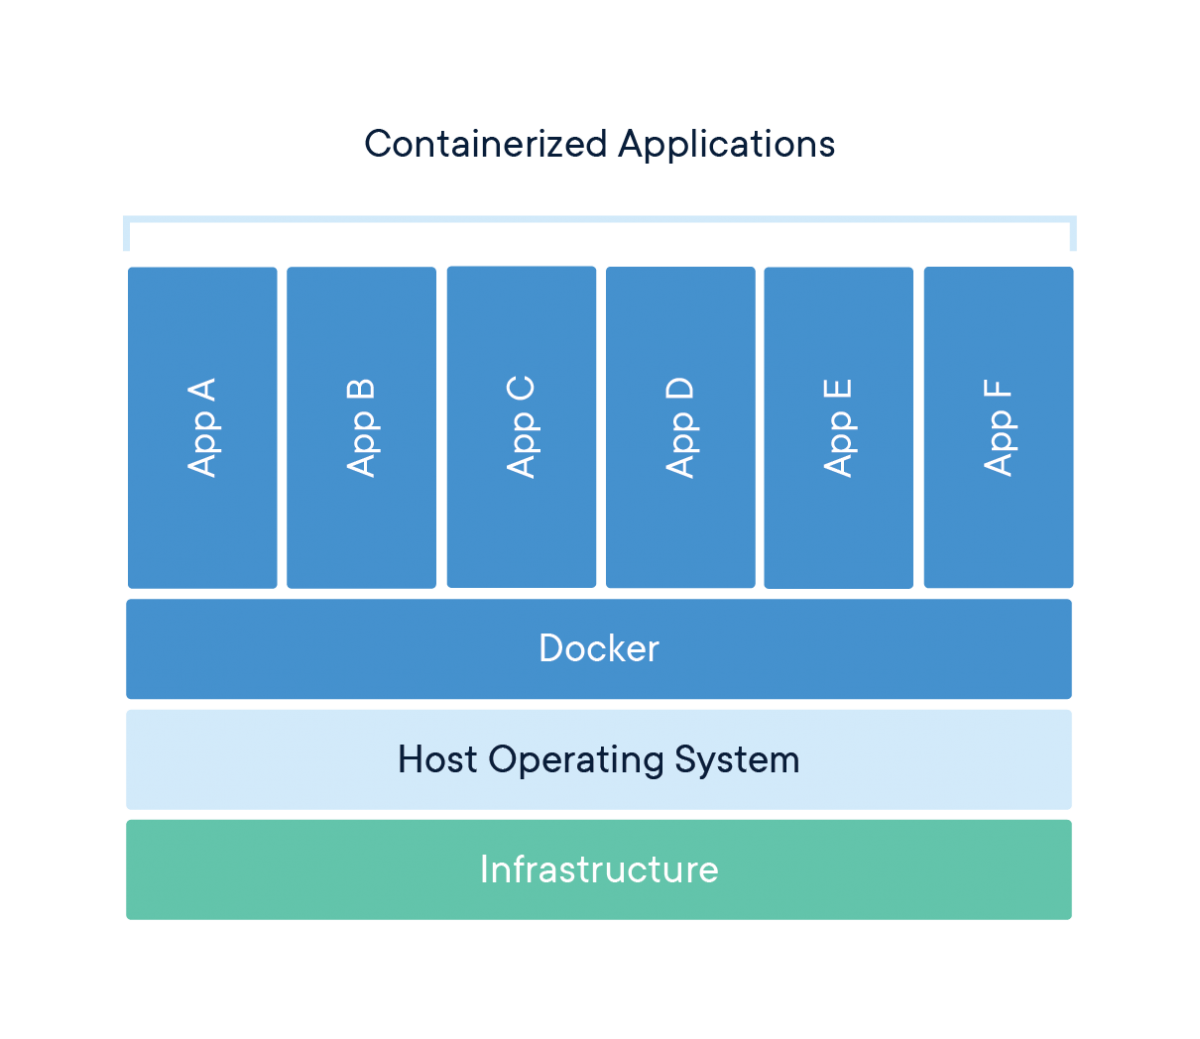
\includegraphics[width=.7\linewidth]{pictures/container-what-is-container.png}
    \caption{Distribución de los contenedores sobre el motor de ejecución de Docker \cite{WhatContainerApp}.}
    \label{fig:docker-containers-rt}
\end{figure}

La distribución de los contenedores mostrada en la figura \ref{fig:docker-containers-rt}
puede parecerse mucho a la distribución que tendríamos en una máquina virtual. Sin embargo,
hay varias características que lo distinguen principalmente:

\begin{enumerate}
    \item Un contenedor se ejecuta directamente sobre la máquina anfitriona, mientras
          que una máquina virtual requiere de un hipervisor.
    \item Un contenedor es una abstracción de la capa de aplicación que encapsula
          el código y las dependencias juntas, mientras que una máquina virtual es
          una abstracción de una capa física \textit{hardware}.
    \item Un contenedor comparte el kernel con el sistema operativo anfitrión, por lo
          que tiene un gran rendimiento; mientras, una máquina virtual ejecutará su
          propio kernel sobre el hipervisor del sistema operativo anfitrión.
    \item El espacio que necesita un contenedor es muy pequeño en comparación con el
          de una máquina virtual, que engloba y encapsula un sistema operativo al
          completo.
\end{enumerate}

\begin{figure}[H]
    \centering
    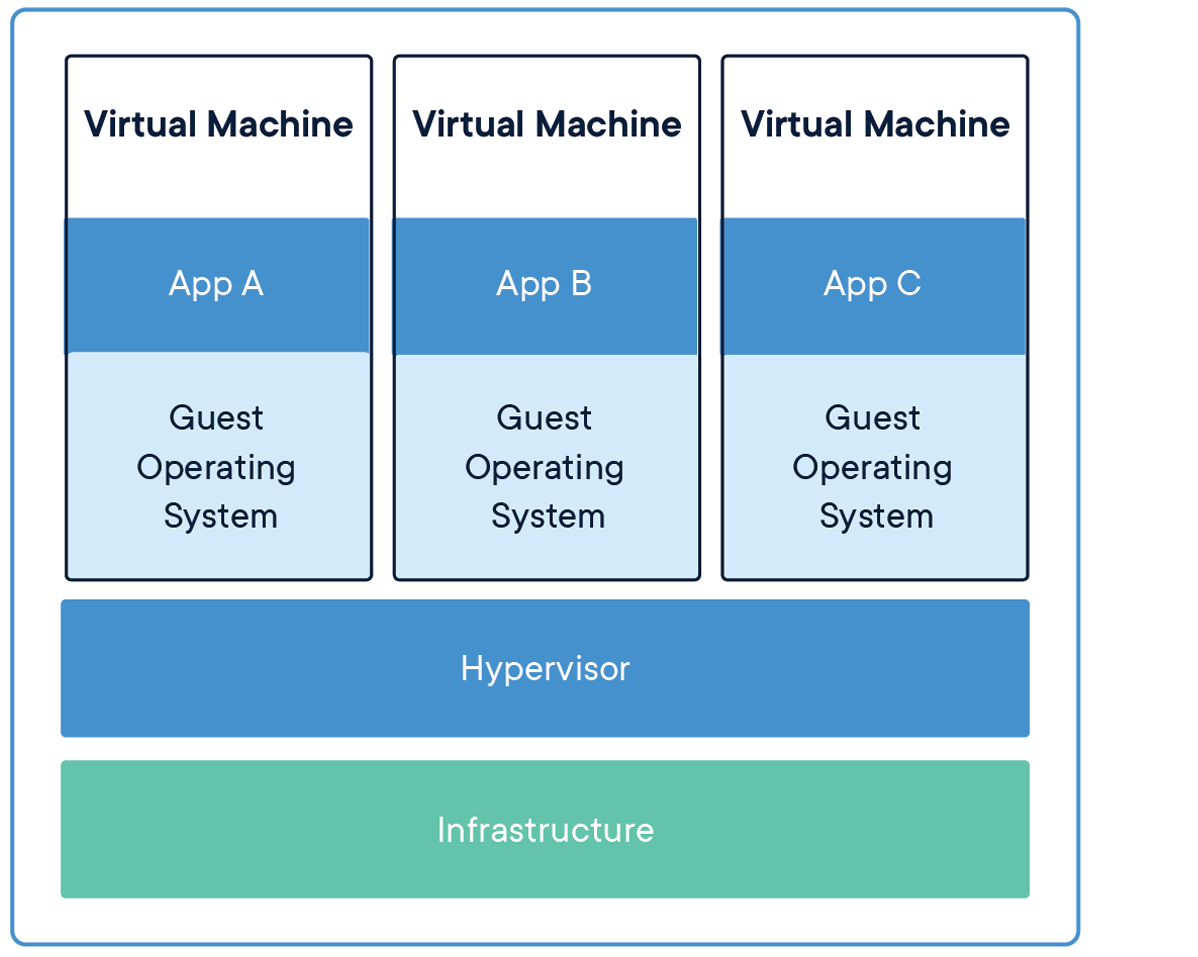
\includegraphics[width=.7\linewidth]{pictures/container-vm-whatcontainer_2.png}
    \caption{Capas de abstracción de una máquina virtual sobre una máquina anfitriona \cite{WhatContainerApp}.}
    \label{fig:vm-layers}
\end{figure}

En la figura \ref{fig:vm-layers} se puede apreciar cómo una máquina virtual añade
muchas más capas de abstracción que ralentizan el rendimiento. Sin embargo, esto
no quiere decir que sean una mala alternativa: la realidad es que se combinan las
dos para obtener una gran flexibilidad para desplegar aplicaciones -- contenedores
cuando se quiere ejecutar algo directamente sobre el anfitrión; máquinas virtuales
para emular \textit{hardware} y que ejecuten en su interior contenedores para ejecutar
aplicaciones fácilmente.

La evolución y constante mantenimiento de los contenedores ha generado lo que se
conoce como estándar de la industria ``\textit{containerd}''. Este estándar define
claramente qué arquitectura debe tener un contenedor por debajo y está en constante
evolución a medida que la industria crece y madura.

Además, la especificación anterior ha pasado de ser un mero estándar a una aplicación
en sí de gestión y orquestación de contenedores, permitiendo que aplicaciones distintas
de Docker hagan uso de la arquitectura basada en contenedores aprovechando la OCI:
\textit{Open Container Initiative}

\begin{figure}[H]
    \centering
    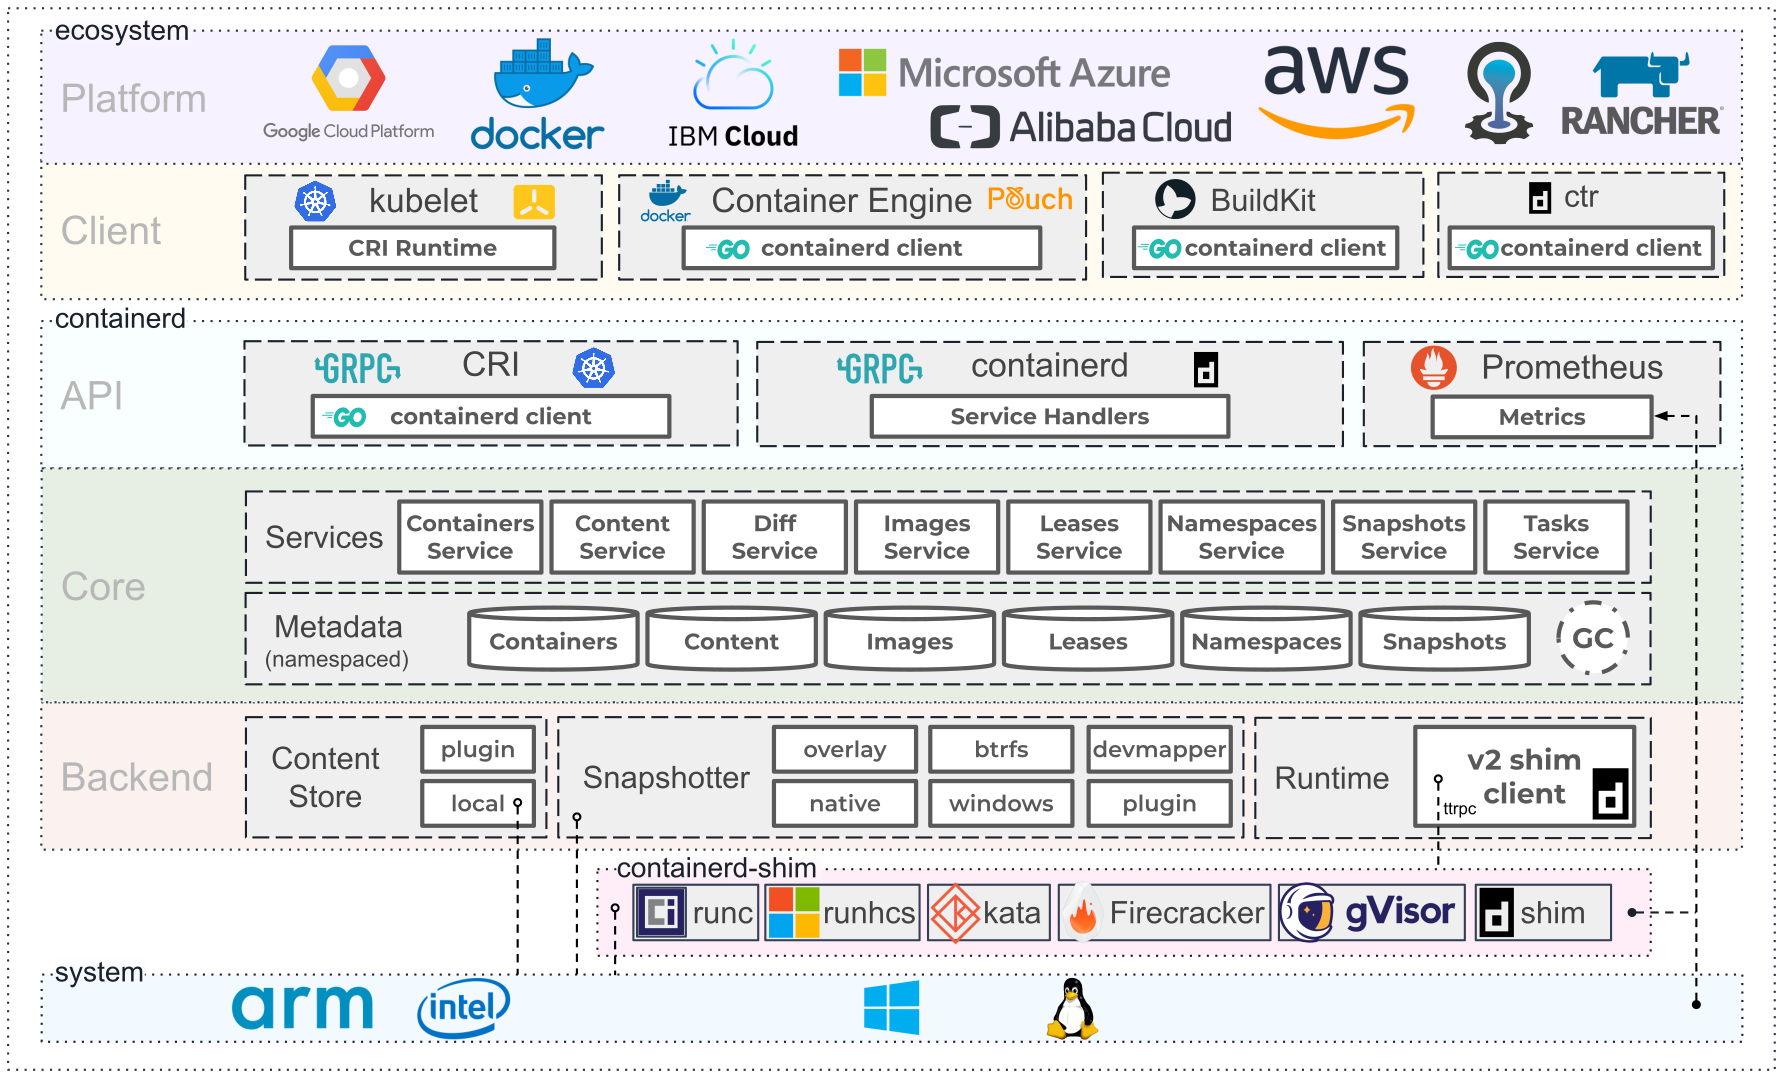
\includegraphics[width=.7\linewidth]{pictures/containerd-arch.png}
    \caption{Entorno de ejecución de \textit{containerd} basado en \texttt{runC} de la OCI \cite{Containerd}.}
    \label{fig:containerd-arch}
\end{figure}

\subsubsection*{Docker Engine}
El motor de ejecución de Docker establece la arquitectura de ejecución \textit{de facto}
que es utilizable desde distintas distribuciones Linux y servidores Windows \cite{ContainerRuntimeDocker}.

\begin{figure}[H]
    \centering
    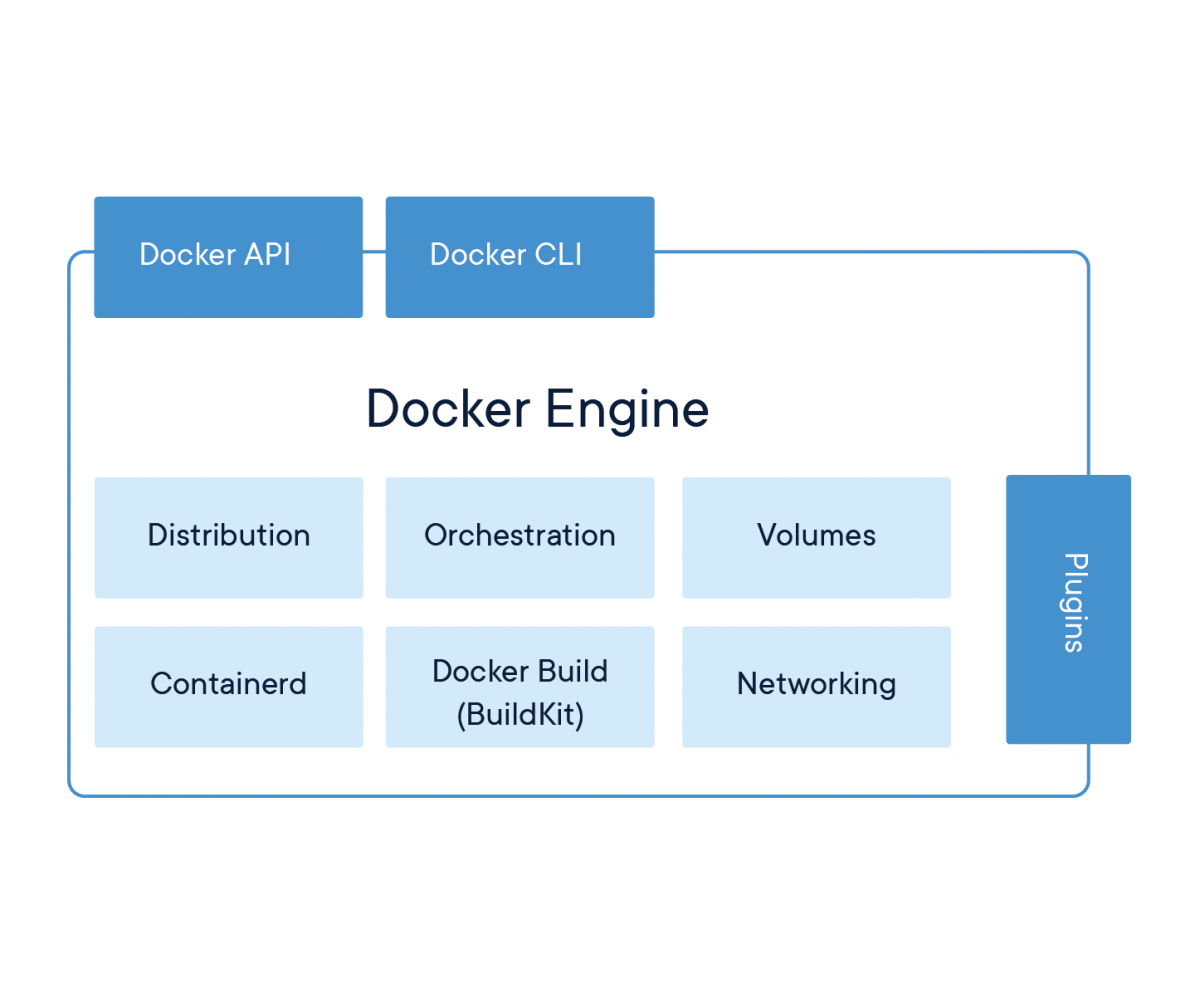
\includegraphics[width=.7\linewidth]{pictures/docker-engine.png}
    \caption{Arquitectura del entorno de ejecución de Docker \cite{ContainerRuntimeDocker}.}
    \label{fig:docker-engine}
\end{figure}

El motor de ejecución de Docker se compone de una gran cantidad de elementos que
encapsulan de forma uniforme multitud de aptitudes de un sistema operativo o una
aplicación (figura \ref{fig:docker-engine}). Este entorno de ejecución sin embargo
es complejo ya que engloba multitud de elementos físicos, como pueden ser las interfaces
de red y los volúmenes.

Esto resulta fundamental ya que los contenedores Docker no tienen ni que confiar en
la red del anfitrión: tienen su propio \textit{stack} de red para realizar las comunicaciones
que necesiten. Con el motor de ejecución de Docker se busca solventar esos problemas
``\textit{dependency hell}'' que se han comentado anteriormente y la situación de ``en mi equipo
funciona''.

De los elementos mostrados en la figura \ref{fig:docker-engine}, se tiene que son:

\begin{itemize}
    \item \textit{Distribution}: la distribución Linux en la que se basa el contenedor.
          Actualmente, Docker solo permite ejecutar contenedores basados en Linux.
    \item \textit{Orchestration}: cuando hay múltiples contenedores, la orquestación
          es el proceso por el cual el motor de ejecución de Docker gestiona y
          maneja qué contenedores se ejecutan, cómo se comunican, cuáles hay que
          crear nuevos y cuáles eliminar. Es de las partes más complejas que existen
          en el mundo de los contenedores y ha evolucionado a clústers mucho más
          completos (y complejos) como Kubernetes o Docker Swarm.
    \item \textit{Volumes}: los volúmenes (conjuntos de datos) que se manejan en los
          contenedores. Debido a su arquitectura cerrada, los datos que genera un
          contenedor solo están visibles para ese contenedor mientras este esté en
          ejecución. Cuando finalice, todos los datos no persistentes son eliminados.
    \item \textit{Containerd}: el estándar y cliente de ejecución y manejo de los
          contenedores a muy bajo nivel.
    \item \textit{Docker Build (BuildKit)}: herramienta de libre distribución que
          transforma los ficheros \texttt{Dockerfile} en imágenes Docker, listas
          para ser usadas y distribuídas.
    \item \textit{Networking}: \textit{stack} de red completo que se pone a disposición
          de cada contenedor Docker. Cada aplicación puede crear su propio dispositivo
          de red que cumpla con los requisitos que necesita. Existen varios tipos de
          adaptadores: \textit{bridge}, \textit{NAT} y \textit{host}. El primero
          se emplea para realizar comunicaciones a través de red entre distintos
          contenedores; el segundo para realizar comunicaciones con el exterior
          mediante una conexión de red completamente independiente a la del anfitrión;
          la tercera para compartir la interfaz de red del anfitrión con el contenedor,
          como si fuese una aplicación interna.
\end{itemize}

Con todo lo anterior, una aplicación puede ejecutarse muy fácilmente en cualquier
equipo que integre el motor de ejecución de Docker.

\noindent\rule{\linewidth}{.2pt}

Con esto, ya sabemos a \textit{grosso modo} qué es Docker, qué ventajas ofrece y cómo
funciona internamente para permitir la ejecución de aplicaciones y contenedores.

\subsection{\textit{Real--life usages}}
Desde que nació en 2013, Docker ha ido creciendo y con ello las aplicaciones
directas que ha encontrado en el mercado.

\subsubsection*{\textit{Sandboxing}}
Una de las principales ventajas que otorgó Docker desde su nacimiento fue el de
aislar las aplicaciones entre sí y, por consiguiente, ofrecer un entorno de
``caja de arena'' (\textit{sandbox}) en donde ejecutar nuestras aplicaciones
(o aplicaciones inseguras) con cierta confianza \cite{yegulalpWhatDockerSpark2019}.

Es cierto que esta característica ya estaba asentada con las máquinas virtuales,
y funcionaba correctamente y de forma efectiva. Sin embargo, el tiempo de despliegue
y lentitud de una máquina virtual hacía que usarlas para este propósito fuese
costoso y no resultase interesante.

Con los contenedores se puede tener un entorno aislado que funciona igual de rápido
que una aplicación nativa con unos tiempos de despliegue y uso de recursos limitado.
Como se ha visto anteriormente, el motor de ejecución de Docker tiene el control sobre
un montón de componentes virtuales y reales que permiten, entre otros, limitar y
restringir el acceso a los recursos \textit{hardware} del dispositivo. Bajo esta
premisa, un contenedor puede usar solo cierta cantidad de CPU, RAM o red y que
cambie en tiempo de ejecución.

\subsubsection*{Portabilidad}
Otra de las características fundamentales de los contenedores es la
capacidad de encapsular un \textit{software} y todas
sus dependencias. Esto convierte a los contenedores en una gran solución portable:
sabemos que si una aplicación funciona en Docker en un equipo Linux, funcionará en
Docker de otro equipo Linux exactamente igual, sin necesidad de realizar ningún
cambio e indiferentemente de la distribución.

Con la llegada de WSL2, el kernel de Linux se introdujo al completo dentro de las
máquinas Windows 10, permitiendo que Docker se pudiera ejecutar de ``forma nativa''\cite{DockerDesktopWSL2021}. Con esto, la limitación anterior
se elimina y los contenedores diseñados para Linux funcionarán también en Windows.

Esto ha tenido una repercusión directa con el auge de los sistemas basados en la
nube, los cuales a veces resultaban complejos y tediosos. Con los contenedores, una
aplicación que un desarrollador ejecuta \textit{on-premise} en su equipo puede
ser fácilmente desplegada a un entorno \textit{cloud} sin necesidad de preocuparse
si cumple los requisitos o instala las dependencias. La única restricción es que el
entorno \textit{cloud} al que se mueva soporte Docker.

\subsubsection*{Arquitectura de composición}
Una gran mayoría de aplicaciones que se ejecutan actualmente están ejecutándose sobre
una pila de aplicaciones: servidor web, base de datos, caché en memoria, gestión de
\textit{logs}, etc. La pregunta es, ¿qué sucedería si se encapsula cada una de esas
aplicaciones en un contenedor?

Así nace la arquitectura de microservicios, tan popular y estandarizada hoy en día.
Un microservicio define un elemento único de una aplicación (que puede ser usado
entre $1 \dots n$ veces) el cual acelera y facilita las labores de desarrollo de una
aplicación. Entre otras ventajas, un microservicio puede ser actualizado, reemplazado,
eliminado o modificado sin afectar al resto de microservicios que componen una
aplicación. Esta alternativa se ha asentado como la solución ideal a las aplicaciones
monolíticas monstruosas, que lo engloban todo (como XAMPP) ya que han demostrado ser
mucho más fáciles de mantener y desarrollar.

\subsubsection*{Escalado y orquestación}
Aprovechando la arquitectura de microservicios y contenedores, existen
técnicas de escalado y orquestación automáticas basadas en Docker y contenedores.

De esta manera, en picos de conexión se despliegan automáticamente más contenedores
que gestionan entre ellos las peticiones entrantes y salientes. Cuando las solicitudes
bajan, los contenedores en deshuso desaparecen para dejar de usar recursos.

Entre las herramientas más sonadas para la gestión de contenedores está
Kubernetes, desarrollado por Google. La idea de orquestación nace a raíz de esta
empresa que empieza a invertir cantidades millonarias de dinero en contenedores porque
le ve un nuevo potencial: las comunicaciones vía Internet de los contenedores.
Hasta ahora solo hemos visto un modelo de arquitectura: un cliente Docker que ejecuta
uno o varios contenedores. Sin embargo, con la aparición de los microservicios y la
orquestación, y dadas las características de red de los contenedores, se abre la
posibilidad de que múltiples clientes Docker en máquinas físicamente distintas puedan
estar ejecutándose de forma simultánea y compartiendo datos entre ellos fácilmente.

Debido a las capas de aislamiento de Docker, esta comunicación no es sencilla: no sirve
con comunicar dos direcciones IP. Sin embargo, utilizando un motor de Docker distribuído
se pueden realizar las conexiones como si de una LAN se tratase, cuando en realidad se
está usando una red \textit{overlay}. Esto se muestra en la figura \ref{fig:docker-network}:

\begin{figure}[H]
    \centering
    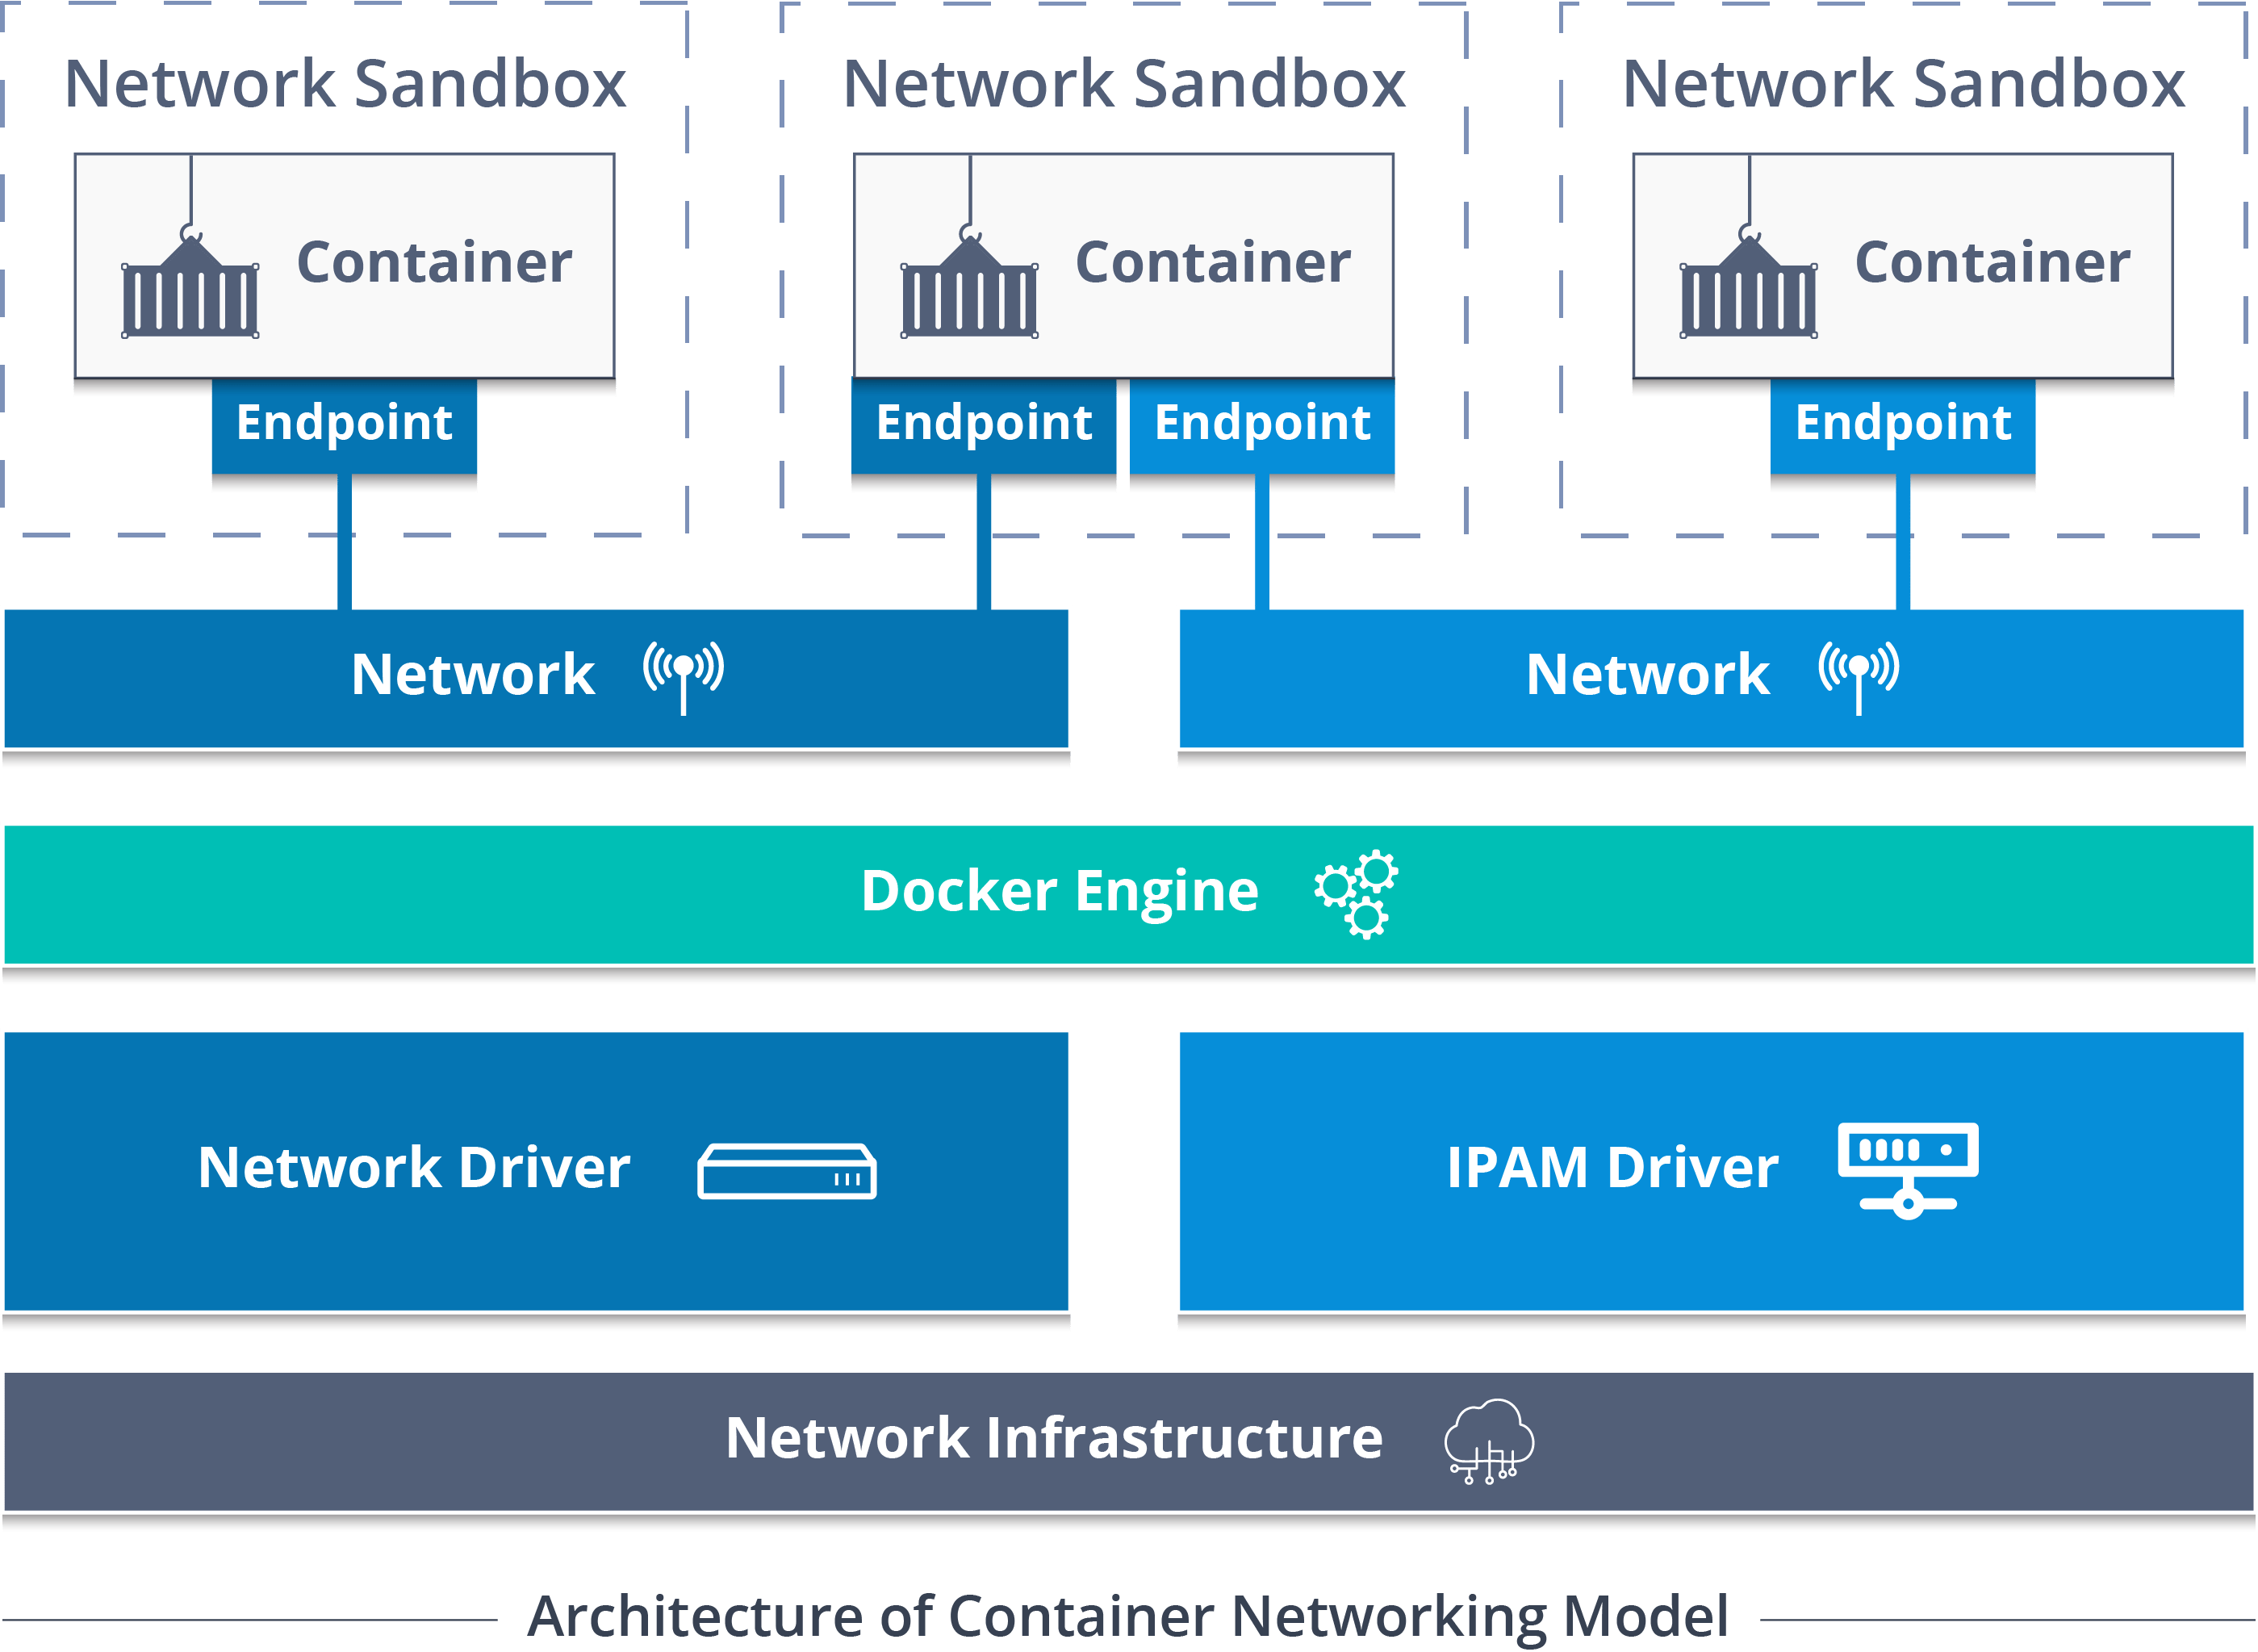
\includegraphics[width=.7\linewidth]{pictures/docker-networking.png}
    \caption{Comunicación entre contenedores usando el motor de Docker \cite{kulshresthaDockerNetworkingExplore2020}.}
    \label{fig:docker-network}
\end{figure}

Con todas estas ideas en mente, es evidente que Docker ofrece soluciones fáciles
y sencillas para escalar automáticamente aplicaciones alrededor de un clúster de
nodos distribuído por el mundo.

\noindent\rule{\linewidth}{.2pt}

Muchas de las aplicaciones de Docker surgen en el mundo DevOps, en donde la mayoría de
herramientas de integración continua (CI) y despliegue continuo (CD) han migrado sus
infraestructuras hacia Docker. Con esto se consigue que los tests y las compilaciones
se hagan de forma sencilla con contenedores de un solo uso.

Otra aplicación directa son las arquitecturas \textit{cloud}, en donde antes había que
configurar cientos de parámetros para desplegar una aplicación web basada en PHP y 
MySQL y ahora basta con usar uno o varios contenedores que agrupen las funcionalidades
que necesitamos.

Por otra parte, gracias a los contenedores los tiempos de desarrollo se han agilizado
mucho. Antes, por ejemplo, una aplicación requería de compilar ciertos paquetes
y realizar ciertas instalaciones que llevaban mucho tiempo. Con Docker, se exponen
las librerías necesarias y se trabaja directamente con aquello que se necesita,
sin necesidad de dedicar tiempo a esas tareas.

\subsection{\textit{Docker rules}}
Desde su nacimiento en 2013 hasta su expansión mundial hace poco más de 4 años, en
2017/18, los contenedores se han convertido en el \textit{modus operandi}
de muchas empresas, que han visto en la tecnología de contenedores una gran ventaja
y forma de despegar y aumentar su producción.

Desde entonces, diversos estudios como el llevado a cabo por Portworx cada año brindan
la oportunidad de ver qué tecnologías dominan el mercado y cómo va evolucionando el
mundo de los contenedores.

De entre los datos obtenidos, es destacable la adopción de contenedores en las
empresas tecnológicas: un 87\% de los encuestados (2019) afirman usar contenedores en
comparación con el 55\% registrado en 2017. Es más, el 90\% de las aplicaciones que
ejecutan en esos contenedores están en entornos de producción, una gran diferencia con
2018 (84\%) y 2017 (67\%) \cite{wattsStateContainersToday}.

Estos datos radican en la inversión económica que las empresas realizan en labores
de ``contenerización'', invirtiendo entre $\$\numprint{500000}$ y $\$\numprint{1000000}$
\cite{wattsStateContainersToday}. De entre todos los motivos que mueven a las empresas
a realizar esas inversiones, prima la seguridad de los datos sobre los demás.

Parece ser que una de las principales labores de los contenedores en estas decisiones
es la de proteger la información (61\%), gestionar las vulnerabilidades fácilmente
(43\%) y proteger el sistema en tiempo de ejecución (34\%). Estos datos van directamente
ligados con las medidas de seguridad que las compañías adoptan al usar contenedores:

\begin{itemize}
    \item Cifrar los datos (64\%).
    \item Monitorización en tiempo de ejecución (49\%).
    \item Escaneo de vulnerabilidades en los registros de contenedores (49\%).
    \item Escaneo de vulnerabilidades en las operaciones de CI/CD (49\%).
    \item Bloquear anomalías mediante la protección en tiempo de ejecución (48\%).
\end{itemize}

El siguiente motivo de la gran adopción de contenedores es que agiliza mucho la
velocidad en el desarrollo y la eficiencia. Por otra parte, la portabilidad de los
contenedores permite a las empresas poder mover sus entornos de producción y
desarrollo entre una y otra plataforma de nube públicas, de entre las cuales las
más usadas (12\% de la muestra) son AWS, Azure y Google Cloud \cite{wattsStateContainersToday}.

En particular, se observa cómo AWS (la plataforma de Amazon) es la dominante en este
sector, llevándose el 78\% del sector; la siguiente, Azure con el 39\%; y finalmente,
GCP (\textit{Google Cloud Platform}) con el 35\% y subiendo rápidamente \cite{ContainerAdoptionTrends}.
Destaca el crecimiento de Google ya que es quien empezó a invertir mucho dinero en
contenedores desde su nacimiento y el creador de Kubernetes, la tecnología de
orquestación más usada a nivel mundial.

\begin{figure}[H]
    \centering
    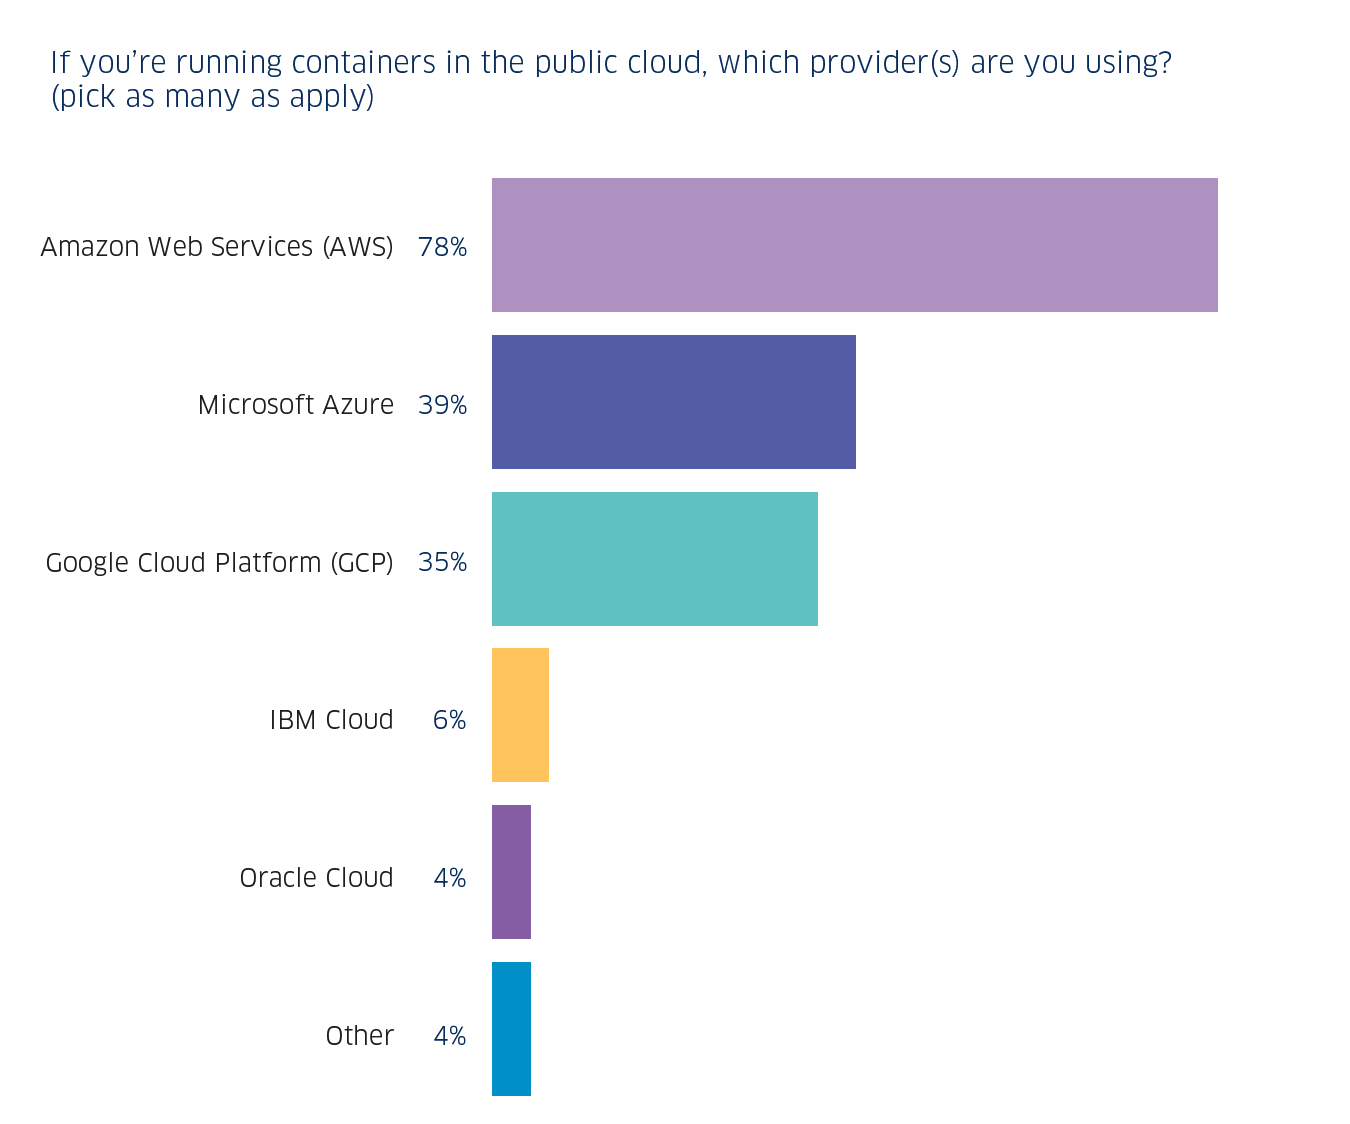
\includegraphics[width=.5\linewidth]{pictures/containers-in-the-cloud.png}
    \caption{Uso de contenedores según la plataforma \textit{cloud} \cite{ContainerAdoptionTrends}.}
\end{figure}

La situación mencionada anteriormente se ve directamente reflejada en la ``contenerización''
de aplicaciones en según que plataforma. De los usuarios de Azure, solo el 20\% ha
creado un contenedor para más de la mitad de sus aplicaciones, significativamente
más bajo que el 33\% de los no usuarios. Esto se ve drásticamente reducido cuando
se hablan de aplicaciones en entorno de producción \cite{ContainerAdoptionTrends}.

Por el contrario, casi un tercio de los usuarios de GCP (31\%) han creado un contenedor
para más de la mitad de sus aplicaciones, relativamente superior al 27\% de los
no usuarios. Este mismo efecto se produce con respecto a las aplicaciones en
producción desplegadas en GCP \cite{ContainerAdoptionTrends}.

Esto se ve reflejado en el gráfico de la figura \ref{fig:contenerized-apps}:

\begin{figure}[H]
    \centering
    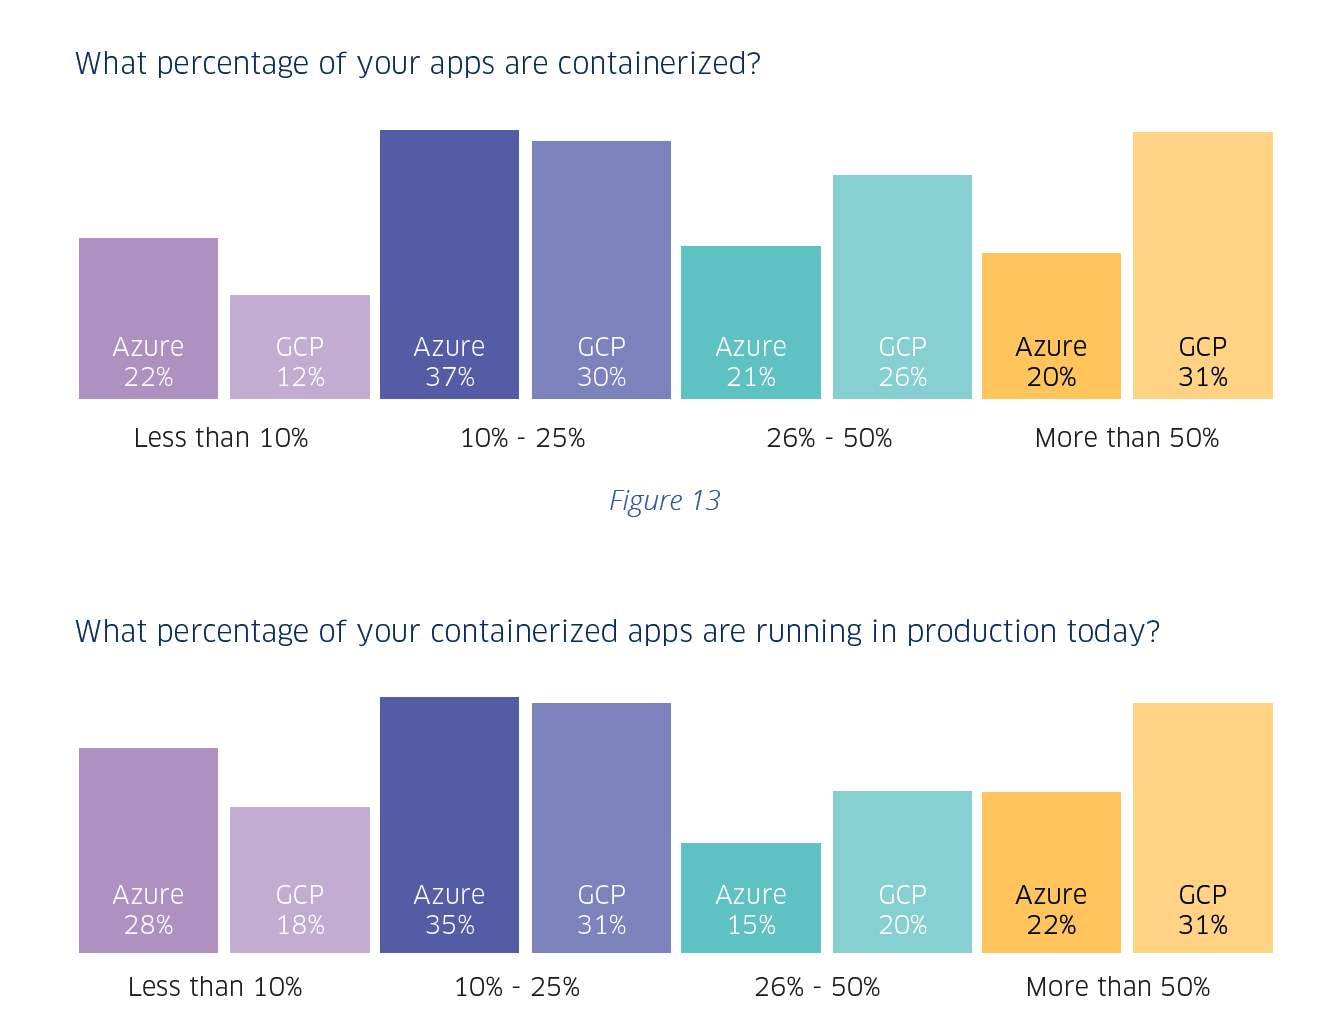
\includegraphics[width=.5\linewidth]{pictures/gcp-vs-azure.png}
    \caption{Porcentaje de las aplicaciones desplegadas en contenedores en según qué plataformas \cite{ContainerAdoptionTrends}.}
    \label{fig:contenerized-apps}
\end{figure}

En un estudio más moderno, se estima en el año 2020 ha supuesto un mayor auge en 
las tecnologías de ``contenerización'', en donde los responsables de IT han priorizado
la creación de contenedores para aplicaciones ya existentes, migrar toda la infraestructura
a la nube y hacer un mejor uso de las plataformas en la nube. De entre todos los
problemas, el principal es cumplir con los requisitos legales, de rendimiento y 
regulatorios vigentes según las necesidades de la industria; y la portabilidad
de las aplicaciones, las cuales estaban confinadas y diseñadas para sistemas en
particular y ahora se quieren desplegar en la nube en general \cite{ContainerAdoptionStatistics}.

Esto se ve en la infografía diseñada por Forrester (figura \ref{fig:container-stats}):

\begin{figure}[H]
    \centering
    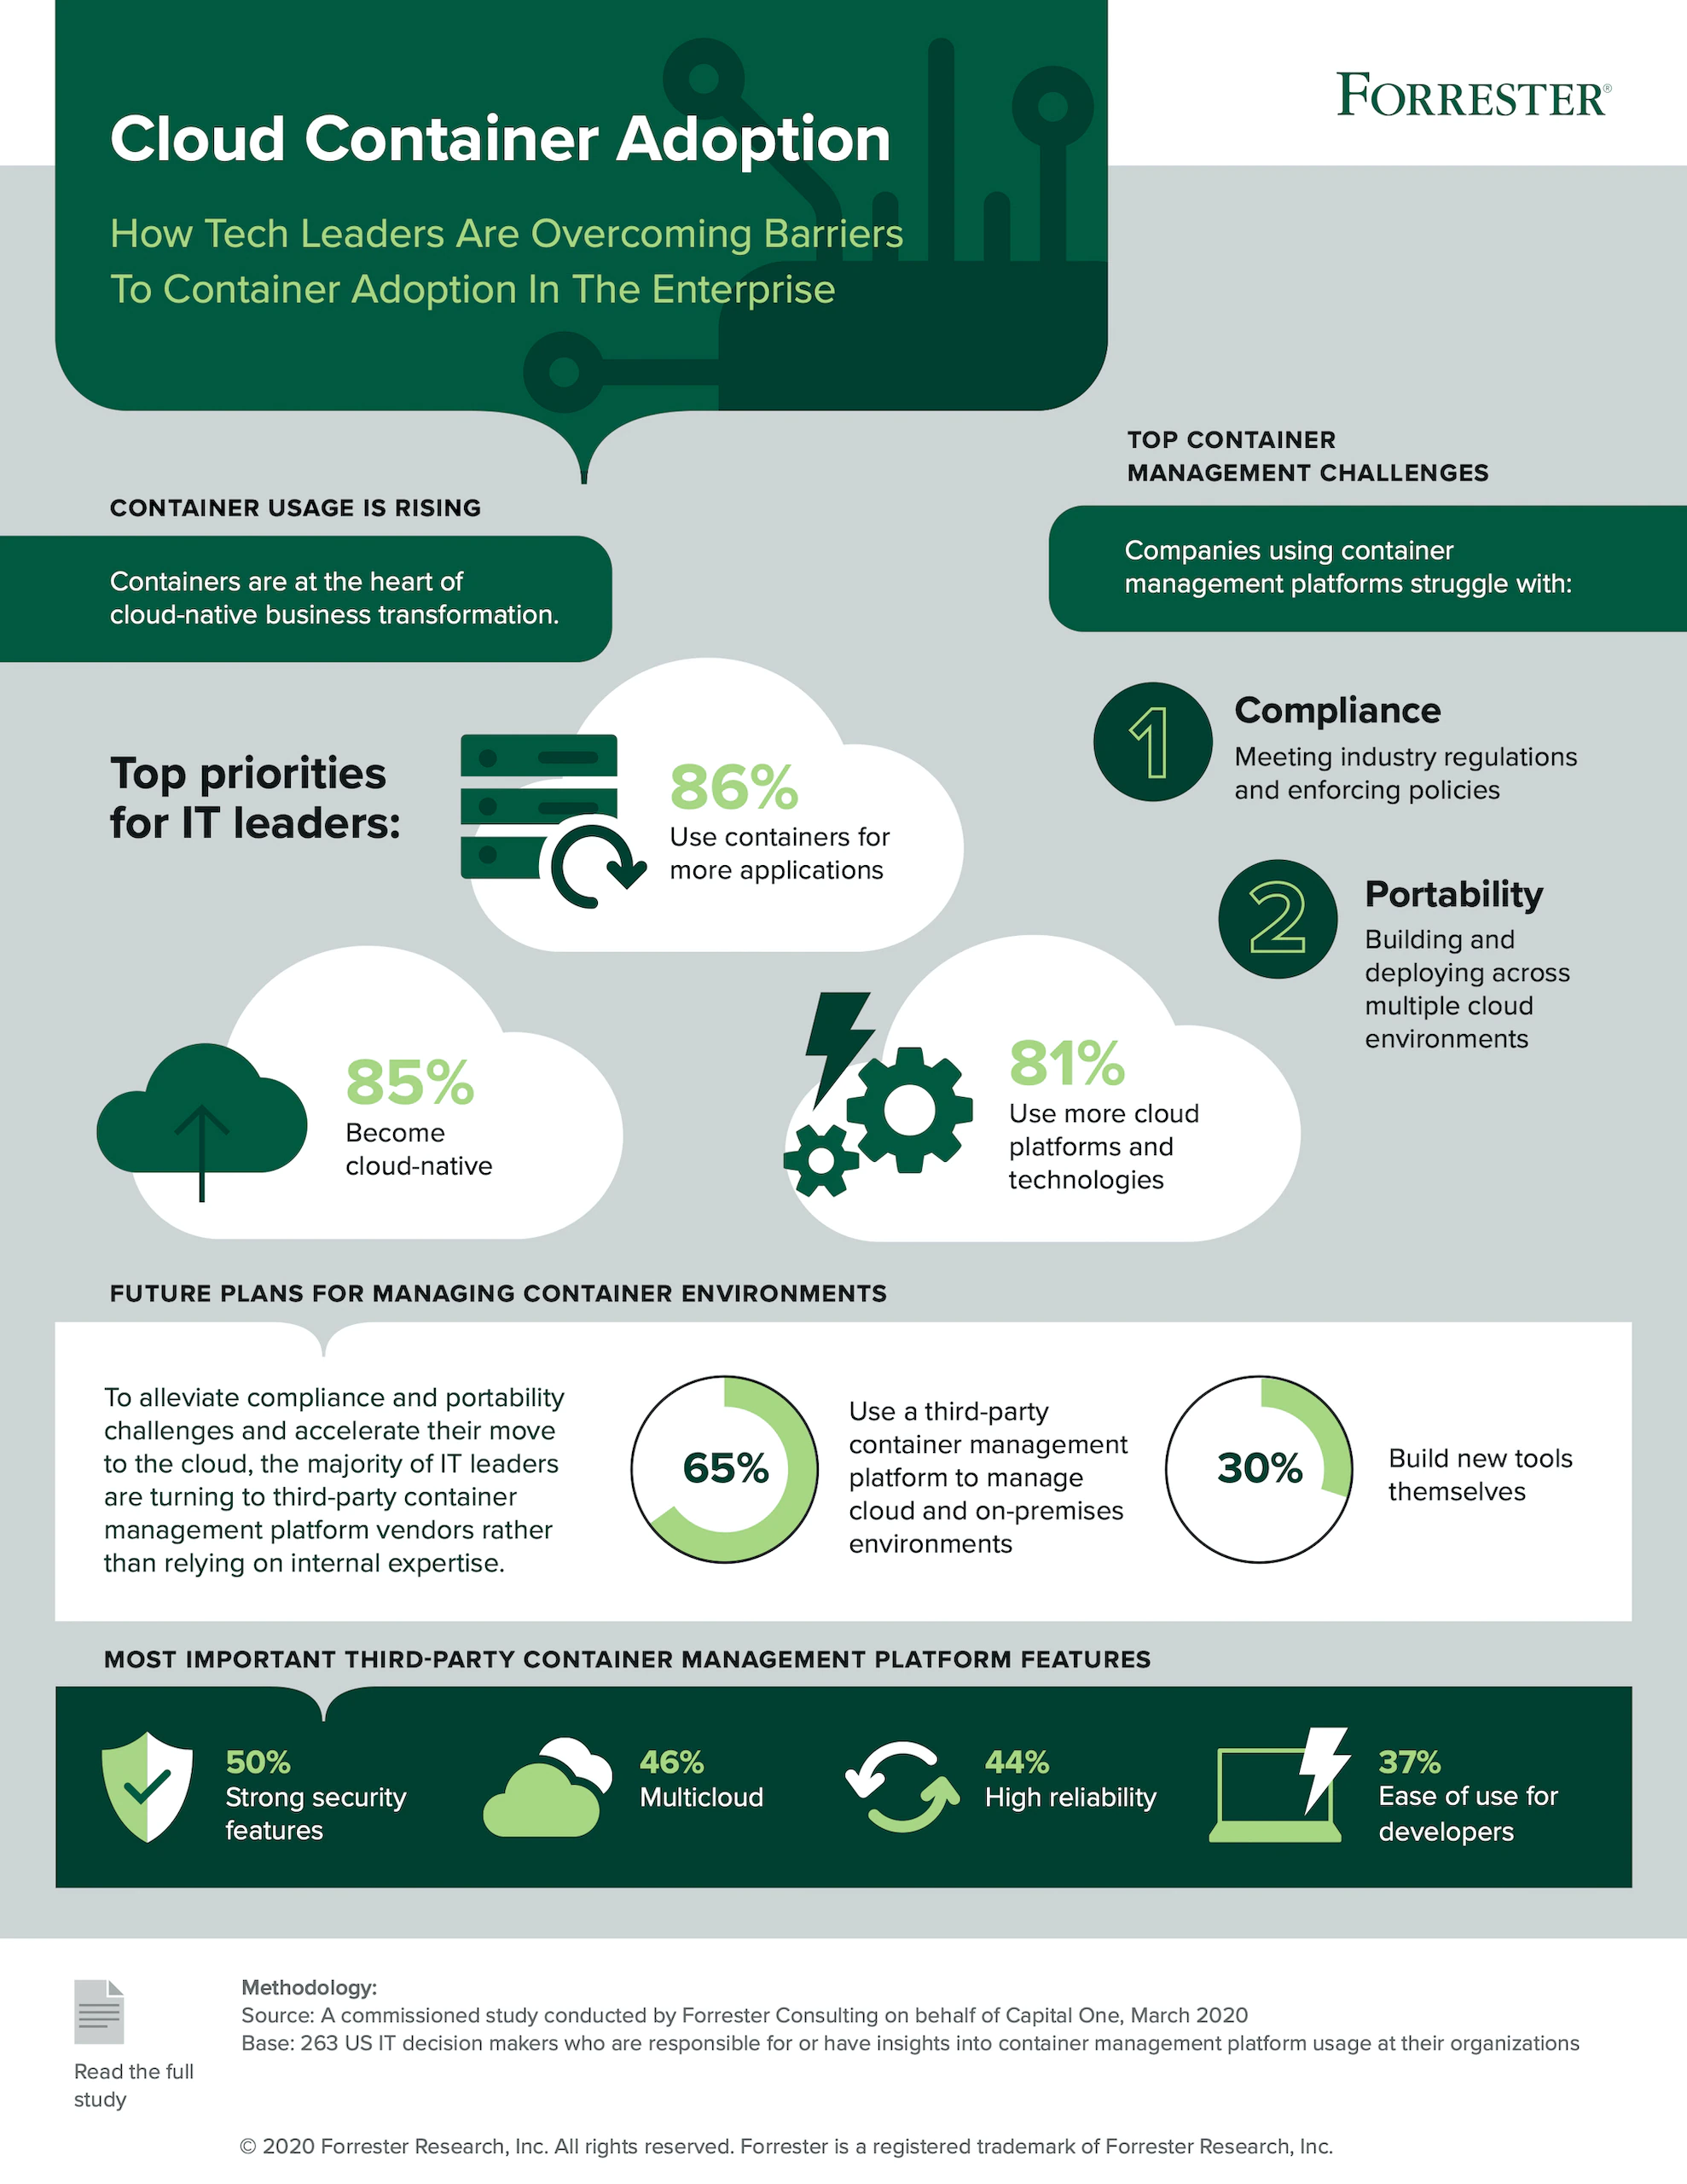
\includegraphics[width=.85\linewidth]{pictures/container-adoption-statistics-infographic.png}
    \caption{Estadísticas de adopción de tecnologías basadas en contenedores en la nube, 2020 \cite{ContainerAdoptionStatistics}.}
    \label{fig:container-stats}
\end{figure}

De entre todos los datos anteriores, es destacable el gran uso de Docker y Kubernetes
para gestionar toda esta infraestructura. En 2017, Docker representaba un 99\% de
los contenedores en uso. Sin embargo, con la compra de CoreOS por RedHat y el
lanzamiento de la OCI ha promovido el nacimiento y establecimiento de nuevas
tecnologías de contenedores que le han quitado cuota de mercado a Docker \cite{Download2018Docker2018}.
Actualmente, la distribución queda (figura \ref{fig:container-runtime}):

\begin{figure}[H]
    \centering
    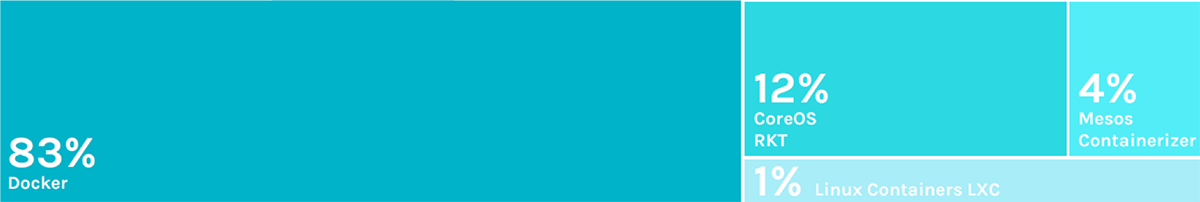
\includegraphics[width=\linewidth]{pictures/container-runtimes.png}
    \caption{Usos de tecnologías de contenedores: Docker domina, seguido por rkt y Mesos \cite{Download2018Docker2018}.}
    \label{fig:container-runtime}
\end{figure}

Todo esto nos lleva a ver que si bien aparecen alternativas nuevas Docker sigue siendo
la tecnología dominante y la que más adopción está teniendo. Esta competitividad es
muy buena ya que permite a Docker y a otras tecnologías de contenedores, como rtk de 
RedHat (CoreOS), evolucionar, seguir avanzando y mejorando. Lo interesante no es ya
usar Docker, rtk o LXC sino que se ha establecido un estándar de contenedores abierto (OCI)
y que pone las bases a lo que es una tecnología revolucionaria.

\section{Docker}
Ahora que ya se han introducido los contenedores, las tecnologías de virtualización
y tendencias de uso, se va a explicar cómo funciona Docker en profundidad. Por una
parte, se va a ver cómo es la estructura de un contenedor Docker, cómo se
comunica con el kernel de Linux, cómo se aísla del resto del sistema y cómo
funciona a nivel de discos virtuales, interfaces de red y gestión de recursos.

Por otra parte, se comentarán diversos ejemplos y estructuras básicas que permiten
la creación de un contenedor aislado, la comunicación de varios contenedores y
el despliegue de una aplicación basada en múltiples contenedores funcionando
simultáneamente.

Finalmente, se comentarán tecnologías de orquestación de contenedores, como son los
clústers de Kubernetes y Docker Swarm y qué planes hay previstos de cara al desarrollo e
innovación de Docker como cliente y gestor de contenedores, para dar pié a un
análisis de la seguridad real de los contenedores, en el punto \ref{sec:security}.
\subsection{Estructura de un Docker}
Docker ofrece un mecanismo de comunicación con un entorno aislado llamado contenedor,
que ha sido introducido anteriormente. Los contenedores por defecto están aislados,
son seguros y empaquetan todo lo necesario para funcionar, por lo que no necesitan
nada del sistema que está por debajo.

Internamente, Docker utiliza la arquitectura ``cliente--servidor'' para gestionar tanto
las comunicaciones y contenedores. Por una parte, el cliente de Docker se comunica
con el \textit{daemon}, el cual es el encargado de realizar las tareas pesadas:
construir (\textit{build}), levantar (\textit{run}) y distribuir (\textit{distribute})
los contenedores Docker.

Lo interesante del servicio en ejecución de Docker es que puede funcionar o bien
en la misma máquina que el cliente o bien sobre otra máquina diferente. Esto es
gracias a que la comunicación del cliente con el servicio se realiza mediante
\textit{sockets} de UNIX, que proveen de una alta velocidad; o bien mediante
interfaces de red, haciendo uso de la API REST de Docker.

\subsubsection*{La arquitectura Docker}

Toda la arquitectura de Docker se puede resumir en la siguiente figura (figura \ref{fig:docker-arch}):

\begin{figure}[H]
    \centering
    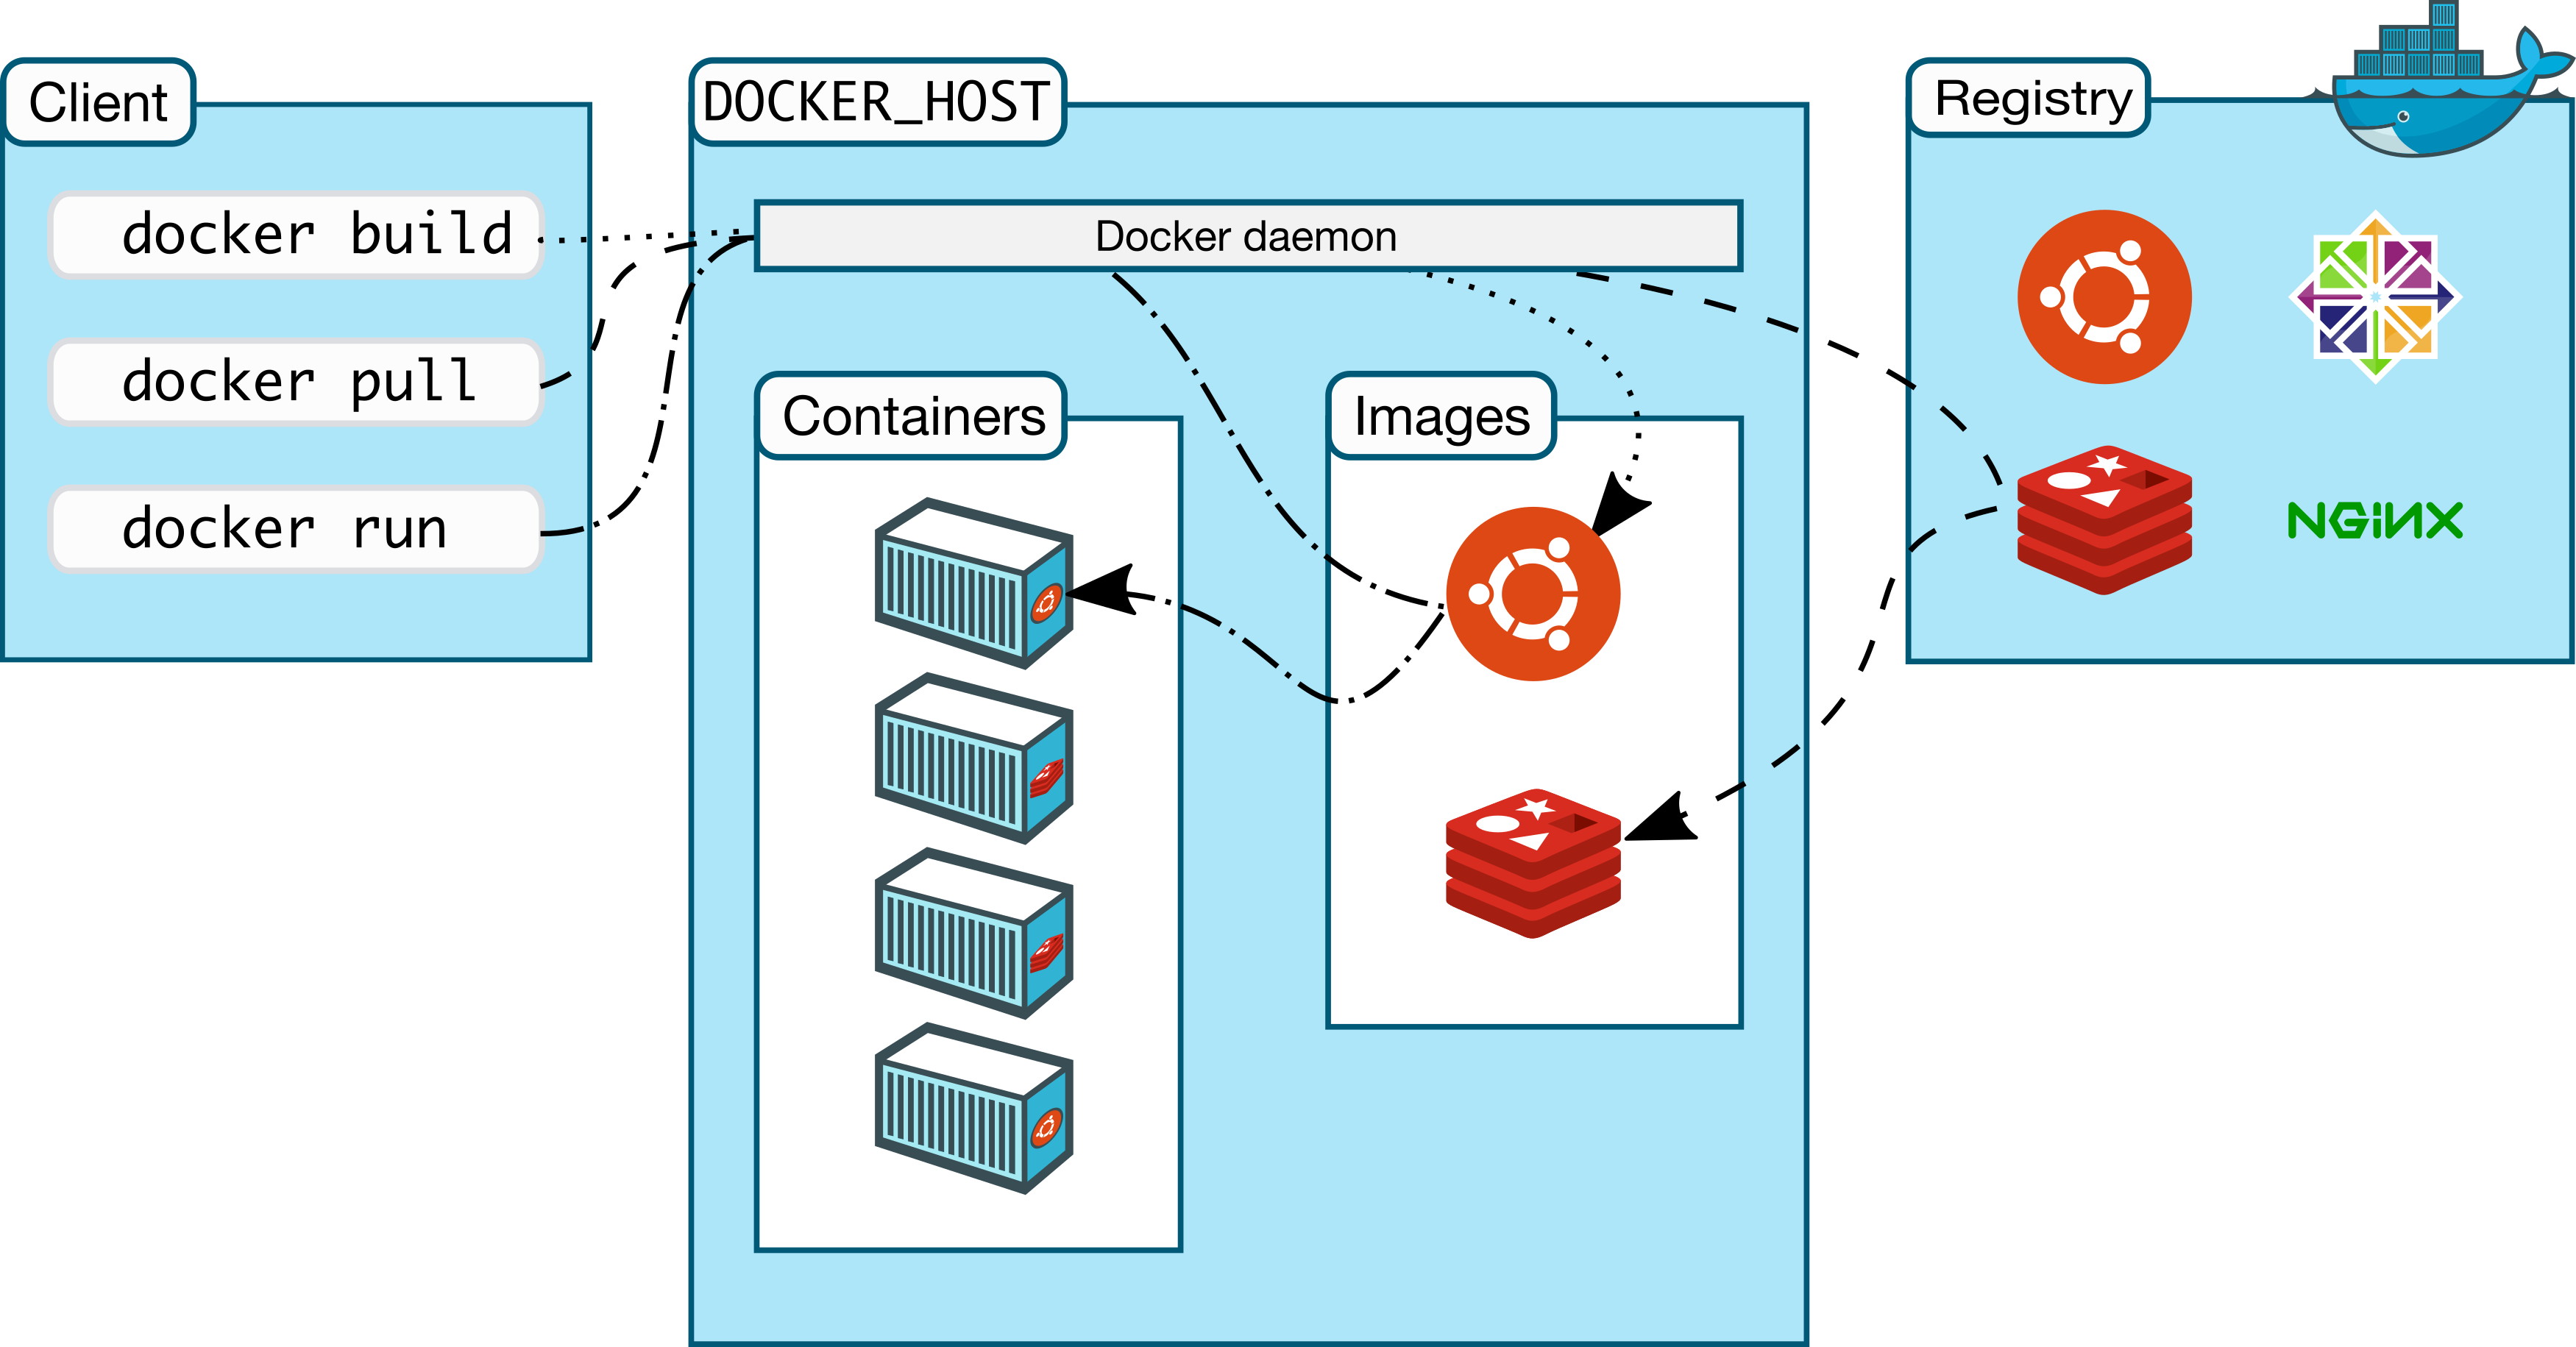
\includegraphics[width=\linewidth]{pictures/docker-arch.png}
    \caption{Arquitectura cliente--servidor de Docker \cite{DockerOverview2021}.}
    \label{fig:docker-arch}
\end{figure}

De la imagen anterior destacan tres bloques principales: el cliente, el servidor
(\textit{docker host}) y el registro (\textit{registry}). Por una parte, el cliente
es la principal forma de comunicarse con el servicio de Docker. Ejecutando comandos
como \texttt{docker run} se envían al servicio peticiones mediante la API REST interna
que gestionan los contenedores.

Por su lado, el servicio está gestionado por el \textit{Docker daemon}, llamado
\texttt{dockerd}. Dicho servicio escucha de forma activa las peticiones API entrantes
y gestiona los objetos de Docker, como las imágenes, contenedores, interfaces de red
y volúmenes. Además, un servicio puede comunicarse con otros servicios para gestionar
a su vez otros contenedores.

Finalmente, los registros de Docker (no confundir con los \textit{logs}, que también
se traduce como ``registro'') son un repositorio en donde se almacenan imágenes Docker.
Por defecto, se hace uso de Docker Hub, que es el registro principal y al cual
el servicio de Docker solicita imágenes cuando no las encuentra, y en donde cualquier
usuario puede publicar la imagen que quiera. Pero, además, una persona puede hospedar
su propio registro privado (al igual que si se desplegase un servidor Nexus).

Uno de los conceptos fundamentales que se han mencionado anteriormente son los ``objetos
Docker''. Esa nomenclatura se usa para agrupar y mencionar a todo aquello que se crea
y genera cuando se trabaja con el servicio de Docker: imágenes, contenedores, interfaces de red,
\textit{plugins}, volúmenes y demás.

\subsubsection*{Imágenes}
Una imagen conforma una plantilla de solo lectura la cual contiene instrucciones
para crear un contenedor Docker. Por lo general, las imágenes se basan en otras
ya existentes con configuraciones adicionales.

Un caso habitual es una imagen basada en \texttt{ubuntu-server} sobre la cual
se instala un servidor Apache y la aplicación NodeJS que hemos desarrollado. Con esto,
tendríamos una imagen la cual se basa en Ubuntu, que ejecuta un servidor Apache y
que tiene una aplicación NodeJS, junto con los ajustes pertinentes para un
correcto funcionamiento, definiendo así una imagen nueva (figura \ref{fig:sample-image}):

\begin{figure}[H]
    \centering
    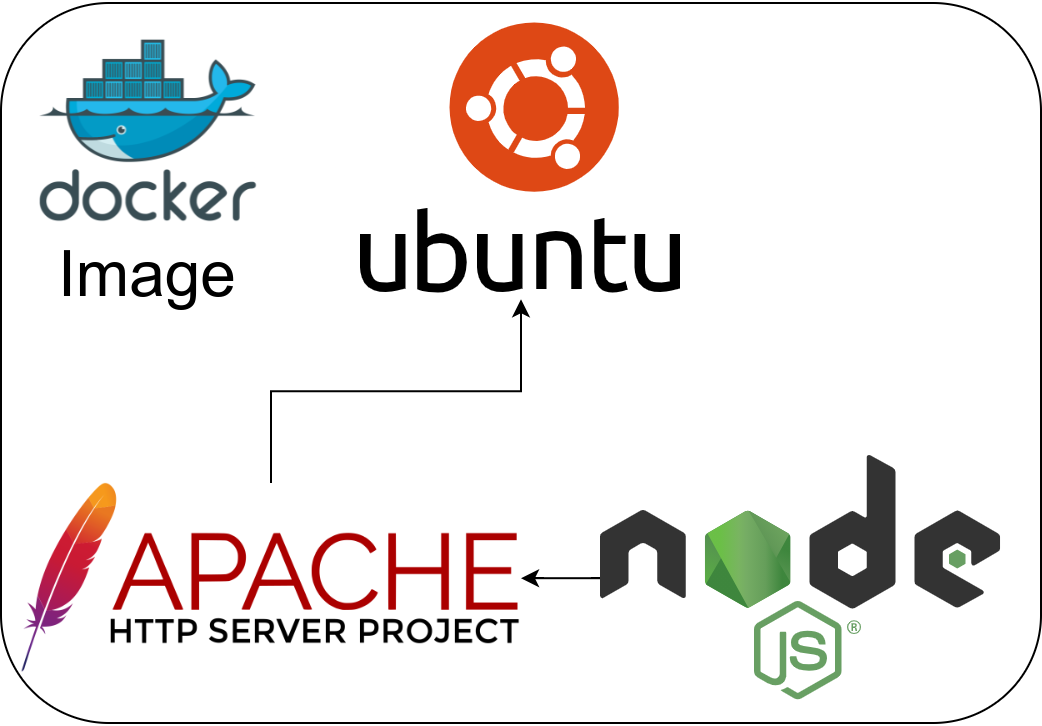
\includegraphics[width=\linewidth]{pictures/sample-image.png}
    \caption{La nueva imagen que habríamos definido basándose en las premisas anteriores.}
    \label{fig:sample-image}
\end{figure}

Cuando se quiere crear una nueva imagen se utiliza un fichero \texttt{Dockerfile}
el cual incluye las directivas necesarias para construir una imagen desde cero (o
basándose en una ya existente). Además, el funcionamiento de este tipo de ficheros
es muy similar a los \texttt{Makefile} en tanto que, cuando se realiza algún cambio
sobre el mismo, solo se reconstruyen en aquellas imágenes que hayan cambiado las
capas modificadas. Esto se traduce en imágenes mucho más pequeñas, ligeras y rápidas
en comparación, por ejemplo, a las máquinas virtuales.

\subsubsection*{Contenedores}
Un contenedor es una instancia de una imagen que puede ser ejecutada. Las operaciones
básicas sobre contenedores son: crear, iniciar, parar, mover o eliminar. Además, se
pueden conectar una o varias redes, volúmenes de datos o inclusive definir y crear
una nueva imagen a partir del estado actual.

Por defecto, un contenedor está bastante bien aislado del resto de contenedores en la
máquina anfitriona. Sin embargo, se puede definir y controlar cómo de aislada está
una red, un almacenamiento o los subsistemas que están por debajo.

Es fundamental tener en cuenta que un contenedor está directamente definido por la
imagen que lo crea y por las configuraciones iniciales que se le dan en el momento
de la creación. Sin embargo, todos los cambios efectuados durante su ciclo de vida
que no sean de imagen o de configuración desaparecerán una vez el contenedor se
detenga y se elimine (esto incluye todo el sistema de ficheros que hay por
debajo).

\subsubsection*{Almacenamiento}
Dada la situación anterior, es necesario buscar alguna manera de persistir la
información de los contenedores. Por defecto, los datos que se generan y gestionan
en un contenedor de Docker son directamente gestionados por el servicio de Docker
y se trabaja con ellos sobre una capa escribible asociada al contenedor \cite{ManageDataDocker2021}.
Esto se traduce en:

\begin{itemize}
    \item Los datos no son persistentes, por lo que eliminar el contenedor eliminará
          la información.
    \item La capa escribible de un contenedor está asociada a dicho contenedor, por
          lo que resulta complejo para otros procesos extraer información de ella.
    \item Además, dicha capa está directamente asociada a la máquina anfitriona en
          donde el contenedor está ejecutándose, por lo que es muy complejo mover
          los datos de un sitio a otro.
    \item Realizar escrituras sobre la capa escribible de un contenedor necesita de
          un driver que gestione el sistema de ficheros. Usando el kernel de Linux,
          este driver ofrece una sistema de ficheros \texttt{UnionFS}, configurado
          a partir de la unión de varios sistemas de ficheros \cite{UnionFS2020}. Esto
          conlleva una penalización en rendimiento en comparación con el uso de volúmenes
          de datos, que trabajan directamente sobre el sistema de ficheros del anfitrión.
\end{itemize}

Por defecto, existen dos formas de persistir los datos de un contenedor: mediante el
uso de volúmenes o mediante \textit{bind mounts}, es decir, asociar un directorio
en el host con un directorio en el contenedor.

\begin{figure}[H]
    \centering
    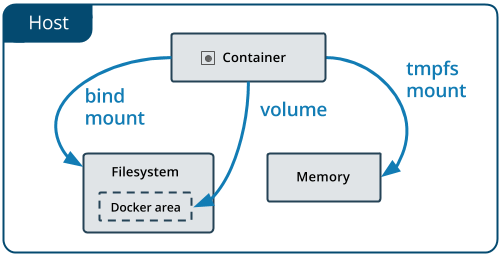
\includegraphics[width=.7\linewidth]{pictures/types-of-mounts.png}
    \caption{Posibles ubicaciones en donde se almacena la información en contenedores Docker \cite{ManageDataDocker2021}.}
\end{figure}

\subsubsection*{\indent --- Volúmenes}
Los volúmenes ofrecen un almacenamiento persistente completamente gestionado por Docker,
por lo que hay que crearlos de forma explícita con ``\lstinline[style=bash]!docker volume create!''.

Cuando se crea un volúmen, los datos se alojan directamente en la máquina anfitriona.
Si se asocia a un contenedor, el volumense monta como un directorio dentro del mismo,
mostrando un funcionamiento similar a \textit{bind mounts}. La principal diferencia
es que los volúmenes ofrecen un entorno completamente aislado de almacenamiento,
gestionado por Docker y portable.

Aprovechando lo anterior, es posible montar un volumen en varios contenedores
abriendo la posibilidad de que compartan datos entre ellos. Además,
los volúmenes son independientes de los contenedores que los usan: si ningún contenedor
usa un volúmen, este sigue existiendo hasta que se elimine manualmente (``\lstinline[style=bash]!docker volume prune!'').

Por otra parte, como los volúmenes son gestionados por Docker permite disponer de
\textit{volume drivers} para almacenar datos en equipos remotos.

Para resumir, se indican las características principales de los volúmenes \cite{UseVolumes2021}:

\begin{itemize}
    \item Son fáciles de manejar, hacer copias de seguridad y de migrar a otros servidores.
    \item Se pueden gestionar completamente desde la interfaz de línea de comandos de Docker.
    \item Funcionan tanto en Windows como en Linux.
    \item Están diseñados para que puedan ser compartidos por varios contenedores de forma segura.
    \item Se pueden almacenar los datos en equipos remotos o proveedores de servicios en la nube.
    \item El rendimiento en plataformas paganas (MacOS y Windows) es mejor que con \textit{bind mounts}.
    \item No incrementan el tamaño del contenedor sino del volumen en sí.
\end{itemize}

Los volúmenes se almacenan en el área de Docker, aislados del sistema dentro del sistema
(figura \ref{fig:volumes-location}):

\begin{figure}[H]
    \centering
    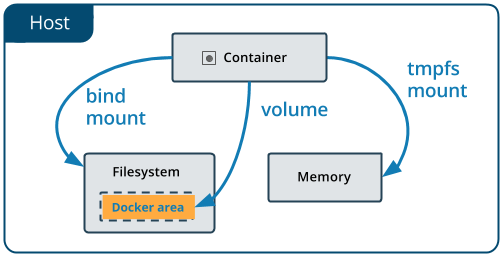
\includegraphics[width=.7\linewidth]{pictures/types-of-mounts-volume.png}
    \caption{Ubicación del almacenamiento de los volúmenes en Docker \cite{UseVolumes2021}.}
    \label{fig:volumes-location}
\end{figure}

\subsubsection*{\indent --- \textit{Bind mounts}}
Los montajes de sistema de ficheros dentro de los contenedores llevan existiendo desde
el lanzamiento inicial de Docker. Su funcionamiento es simple: utilizando los
mecanismos de los sistemas operativos anfitriones, un directorio (o fichero)
en el equipo anfitrión se monta dentro del contenedor en una ruta en específico.
Si el fichero o directorio no existe, se crea bajo demanda en el momento de la
creación del contenedor.

Es importante tener en cuenta que este tipo de sistema de ficheros está mucho más
limitado que un volumen y pueden suponer un gran fallo de seguridad en tanto a que
es posible acceder a ficheros sensibles del sistema.

Hay que tener en cuenta que los contenedores Docker siempre se ejecutan como
súper usuario (administrador), por lo que un proceso malicioso podría editar,
modificar, leer y eliminar ficheros fundamentales del sistema anfitrión si no
se ha tenido cuidado con el directorio a montar.

Sin embargo, es una opción muy interesante para almacenar datos que son modificados
con cierta regularidad o que no interesa ``persistirlos''. Por ejemplo, ficheros
de configuración (para cambiarla bajo demanda), directorios que contengan \textit{logs},
etc.

Los \textit{bind mounts} se almacenan en el sistema de ficheros anfitrión (figura \ref{fig:bind-location}):

\begin{figure}[H]
    \centering
    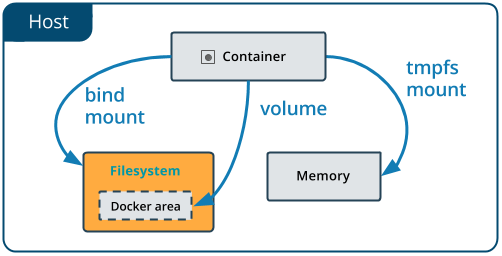
\includegraphics[width=.7\linewidth]{pictures/types-of-mounts-bind.png}
    \caption{Ubicación del almacenamiento de los \textit{bind mounts} en Docker \cite{UseBindMounts2021}.}
    \label{fig:bind-location}
\end{figure}

\subsubsection*{\indent --- ¿Cuándo usar volúmenes o \textit{bind mounts}?}
Basándose en la documentación oficial de Docker \cite{ManageDataDocker2021}, hay
unos casos para unos o para otros, según se requiera (tabla \ref{tab:mount-cases}):

\newpage

\begin{landscape}
    \begin{table}[H]
        \centering
        \begin{tabularx}{\linewidth}{C{.25}||C{.25}|C{.25}|C{.25}|C{.25}|C{.25}|C{.25}|C{.25}}
                                          & \textbf{Compartir datos entre contenedores} & \textbf{Gestionar ajustes} & \textbf{Estructura del FS} & \textbf{Copias de seguridad} & \textbf{Datos en la nube}                                     & \textbf{Alto rendimiento}                              & \textbf{Versiones del código fuente} \\
            \hline
            \textbf{Volúmenes}            & \cmark                                      & \xmark                     & \cmark                     & \cmark                       & \cmark (nativo)                                               & \cmark (en Docker Desktop)                             & \xmark                               \\
            \hline
            \textbf{\textit{Bind mounts}} & \xmark                                      & \cmark                     & \xmark                     & \xmark                       & \cmark (usando un sistema de ficheros en la nube, como SAMBA) & \cmark (depende del sistema de ficheros del anfitrión) & \cmark                               \\
            \hline
        \end{tabularx}
        \caption{Cuándo usar un tipo de almacenamiento persistente u otro, de elaboración propia basándose en la documentación \cite{ManageDataDocker2021}.}
        \label{tab:mount-cases}
    \end{table}
\end{landscape}

\subsubsection*{Interfaces de red}
Docker ofrece un potente mecanismo de gestión de redes para permitir la comunicación
entre contenedores y con elementos externos. Una de las motivaciones principales
detrás de la gestión propia de la red por parte de Docker es la de que las aplicaciones
no sepan si están dentro de un contenedor o si tienen que comunicarse con el exterior
o con una carga de trabajo externa a Docker, sino que van a comunicarse directamente
sin necesidad de ninguna configuración externa.

Indiferentemente de si el servicio se está ejecutando en una máquina Linux y otro en
una máquina Windows, la comunicación entre ellas se va a realizar completamente
independiente a la plataforma.

La gestión de las redes y aislamiento de las mismas se realiza mediante una
manipulación directa de \texttt{iptables}. Esto se hace así porque el \textit{firewall}
nativo de Linux tiene una grandísima potencia, es muy configurable y se ejecuta
directamente a nivel de kernel, lo cual reduce el \textit{overhead} que pudiera
presentar si fuese una aplicación a nivel de usuario.

Esto conlleva que las rutas del \textit{firewall} que se hubiesen creado previamente
deben aparecer antes de las creadas por Docker (para que tengan mayor peso) y 
permiten llevar la ejecución de contenedores Docker a distintos tipos de \textit{hardware}:
servidores, routers (en donde Docker actúa como router) y equipos embebidos.

Por defecto, Docker expone los siguientes drivers \cite{NetworkingOverview2021}:

\begin{itemize}
    \item \texttt{bridge}: el driver que se usa por defecto, si no se especifica 
          ninguno. Se destina este tipo de driver cuando las aplicaciones se
          ejecutan de forma aislada y solo necesitan comunicarse con el exterior o,
          si por el contrario, hace falta que múltiples contenedores se comuniquen
          entre sí.

    \item \texttt{host}: elimina el aislamiento de red con el sistema anfitrión,
          usando la interfaz del sistema (por lo que se debe ajustar
          el \textit{firewall} y la red, si necesita alguna característica especial).
        
    \item \texttt{overlay}: interconecta múltiples servicios de Docker (que pueden
          estar en máquinas distintas) para facilitar la comunicación entre clústers
          de Docker Swarm o contenedores entre sí.

    \item \texttt{macvlan}: asigna una dirección MAC al contenedor de forma que parezca
          que es una máquina física, por lo que se realiza el enrutamiento según las
          direcciones MAC.

    \item \texttt{none}: deshabilita todas las comunicaciones de red para el
          contenedor, se suele usar conjunto a un driver personalizado.

    \item \textit{Network plugins}: cada persona puede desarrollar su propio
          driver de red para que cumpla con una función específica.
\end{itemize}

\subsection{Creación de un contenedor}
La creación de un contenedor siempre se realiza de la misma manera: mediante un
fichero \texttt{Dockerfile}. Los \texttt{Dockerfile} son ficheros del estilo de
los \texttt{Makefile} que contienen unas reglas básicas que definen lo que será
una imagen de un contenedor.

El comando que crea una imagen es \lstinline[style=bash]!docker build!, el cual
toma las instrucciones que aparecen en el fichero y las va ejecutando una a una
hasta que se produce un error o finaliza correctamente.

Un fichero \texttt{Dockerfile} cuenta con multitud de directivas que permiten
personalizar y configurar cómo va a funcionar \cite{DockerfileReference2021}.
Aquí se van a introducir algunas de las más importantes (o las más usadas) \cite{jethvaHowDockerfileWorks}:

\begin{itemize}
    \item \texttt{FROM}: define una imagen base de partida sobre la que construir.
    \item \texttt{ADD}: copia ficheros y directorios dentro de la imagen del 
          contenedor. Además, acepta URLs como parámetro y las descarga
          directamente dentro.
    \item \texttt{RUN}: añade capas a la imagen base, instalando aplicaciones,
          librerías y componentes.
    \item \texttt{CMD}: especifica qué comandos se deben ejecutar al iniciarse
          el contenedor. Es importante tener en cuenta que solo puede existir una
          instrucción \texttt{CMD} en el fichero \texttt{Dockerfile} (si no, se usa solo
          el último que aparezca). Su funcionalidad principal
          es la de establecer los valores por defecto de un contenedor en ejecución.
    \item \texttt{ENTRYPOINT}: es la instrucción ``principal'' de un \texttt{Dockerfile}.
          Especifica el punto de entrada de un contenedor que se quiere que funcione como
          un ejecutable. Por ejemplo, el siguiente comando ``\lstinline[style=bash]!docker run -it --rm -p 80:80 nginx!''
          ejecuta un servidor NGINX de forma interactiva, publica el puerto 80 y, cuando finaliza
          su ejecución, se elimina.
    \item \texttt{ENV}: define las variables del entorno del contenedor que se usarán
          en tiempo de ejecución.
    \item \texttt{COPY}: con una funcionalidad similar a \texttt{ADD} pero con
          más limitaciones.
    \item \texttt{EXPOSE}: define en qué puertos la aplicación estará escuchando.
    \item \texttt{USER}: especifica el UID (o el nombre del usuario) que se usará
          internamente en el contenedor para ejecutar las aplicaciones.
    \item \texttt{VOLUME}: define volúmenes de datos a crear o un punto de montaje del
          contenedor en tiempo de ejecución.
    \item \texttt{WORKDIR}: especifica la ubicación en donde se ejecutará el comando
          en tiempo de ejecución.
    \item \texttt{LABEL}: especifica etiquetas del contenedor en forma de metadatos.
          Se conforman de parejas clave--valor que especifican información relativa
          a la imagen dentro del contenedor como, por ejemplo, la versión, el nombre
          del paquete, etc.
\end{itemize}

Por lo general, un \texttt{Dockerfile} comienza con la especificación de una imagen
de partida (ya que no es habitual crear una imagen desde cero) y, a continuación, se
procede a instalar diversos paquetes y capas que puedan ser necesarias para nuestra
aplicación. A continuación se copian los paquetes y requisitos de la aplicación
dentro de la imagen y se ejecuta la compilación o preparación del paquete, si
fuera necesario. Finalmente, se especifica el punto de entrada del contenedor y
los argumentos que recibirá, si recibe. Además, si es necesario se añaden los puertos
expuestos y volúmenes necesarios para el funcionamiento.

En el código \ref{lst:dockerfile-example} se tiene un ejemplo de un \texttt{Dockerfile}
completo \cite{BestPracticesWriting2021}:

\begin{lstlisting}[style=Dockerfile, caption={Ejemplo de \texttt{Dockerfile} para una aplicación Go \cite{BestPracticesWriting2021}.}, label={lst:dockerfile-example}]
# syntax=docker/dockerfile:1
FROM golang:1.16-alpine AS build

# Install tools required for project
# Run `docker build --no-cache .` to update dependencies
RUN apk add --no-cache git
RUN go get github.com/golang/dep/cmd/dep

# List project dependencies with Gopkg.toml and Gopkg.lock
# These layers are only re-built when Gopkg files are updated
COPY Gopkg.lock Gopkg.toml /go/src/project/
WORKDIR /go/src/project/
# Install library dependencies
RUN dep ensure -vendor-only

# Copy the entire project and build it
# This layer is rebuilt when a file changes in the project directory
COPY . /go/src/project/
RUN go build -o /bin/project

# This results in a single layer image
FROM scratch
COPY --from=build /bin/project /bin/project
ENTRYPOINT ["/bin/project"]
CMD ["--help"]
\end{lstlisting}

En el fichero anterior se establece una imagen de partida \texttt{golang:1.16-alpine}
que contiene los binarios de Go en una distribución de muy poco peso (proyecto Linux
Alpine). Esta imagen se obtiene desde \href{https://hub.docker.com/_/golang}{Docker Hub}.

A continuación, instala el paquete \texttt{git} y el gestor de dependencias de Go.
Después, copia el proyecto en sí e instala las dependencias en la ruta \texttt{/go/src/project}.
Finalmente, copia el directorio actual en dicha ruta y define una nueva imagen partiendo
de la de Golang en donde se ejecuta el proyecto compilado con las opciones
\texttt{-{}-help} por defecto.

Cuando se define un contenedor es recomendable instalar solo aquellas dependencias
que sean necesarias. Esto permite una mayor y mejor mantenibilidad, reduce la complejidad
y el tiempo de construcción de la imagen.

Por otra parte, se recomienda encarecidamente desacoplar la aplicación: por ejemplo,
un servidor web posiblemente requiera de varias aplicaciones en ejecución. Es recomendable
separarlas en contenedores y habilitar la comunicación entre ellos a encapsularlo todo
en un único contenedor. Esto facilita, entre otros, un escalado horizontal en donde
si se requieren de más imágenes se crean.

Además, el número de capas se debe mantener lo más pequeño posible: las instrucciones
\texttt{RUN}, \texttt{COPY} y \texttt{ADD} crean capas, mientras que otras instrucciones
solo crean imágenes intermedias.

Finalmente, es importante construir el \texttt{Dockerfile} teniendo en cuenta que Docker
usa una caché interna. Si se quiere deshabilitar se puede hacer con la opción
\lstinline[style=bash]!--no-cache=true! en el comando \lstinline[style=bash]!docker build!.
Sin embargo, es recomendable hacer uso de la caché interna de Docker ya que agiliza
el proceso de construcción.
\subsection{Comunicación entre contenedores}
\subsection{Despliegue de aplicaciones multi--contenedores. \texttt{docker-compose}}
\subsection{``Orquestación'' de contenedores}
\subsection{Líneas futuras de desarrollo e innovación}

\section{Seguridad en Docker}\label{sec:security}
\subsection{Análisis de la pila Docker}
\subsection{Diferencias fundamentales con \texttt{chroot}}
\subsection{Seguridad en las comunicaciones de red -- \textit{firewall}}
\subsection{Seguridad en las comunicaciones inter--contenedores}

\printbibliography[heading=bibintoc]

\appendix

\end{document}